\documentclass{rapportENSIAS}

\usepackage{lipsum}
\usepackage{minted}
\definecolor{bg}{rgb}{0.95,0.95,0.95}

\usepackage{titlesec}
\usepackage{tocloft}
\usepackage{hyperref}
\usepackage{enumitem}
\usepackage{array}
\usepackage{graphicx}
\usepackage{longtable}

% Espacement des lignes dans les tableaux
\renewcommand{\arraystretch}{1.4}

\title{Rapport de Stage d'Été - Gestion du parc informatique}

\begin{document}

%----------- Informations du rapport ---------

\titre{Conception et développement d'une application web de gestion du parc informatique}
\sujet{Projet de Stage d'Été}
\enseignant{Mehdi Sabri}
\eleves{Adam Achamli}
\jury{}

%----------- Initialisation -------------------

\fairemarges
\fairepagedegarde


%================================================
% REMERCIEMENTS
%================================================

\chapter*{Remerciements}
\addcontentsline{toc}{chapter}{Remerciements}

Je remercie d’abord Dieu le Tout-Puissant, source de force, de patience, de santé et de persévérance, qui m’a guidé tout au long de ce stage et m’a permis d’achever ce travail dans de bonnes conditions.

J’exprime ensuite ma profonde gratitude à mon encadrant, Monsieur Mehdi Sabri, pour son accompagnement précieux, ses conseils avisés, ses remarques constructives et son soutien constant durant la période de stage. Son encadrement a contribué de manière significative à la qualité de ce projet.

Je tiens également à remercier l’École Nationale Supérieure d’Informatique et d’Analyse des Systèmes (ENSIAS) pour l’environnement académique, les enseignements et les compétences qu’elle m’a transmis, ainsi que pour l’opportunité de réaliser ce stage d’été dans un cadre professionnel stimulant.

Je remercie chaleureusement l’équipe de Norsys Afrique pour son accueil, sa disponibilité, son écoute et les informations utiles qu’elle m’a fournies concernant les besoins et les contraintes réelles du parc informatique. Cette expérience m’a permis de mieux comprendre le fonctionnement d’un environnement professionnel et de me familiariser avec les enjeux de gestion, de sécurité et d’innovation numérique.

Enfin, j’adresse mes sincères remerciements à toutes les personnes qui ont contribué, de près ou de loin, à la réalisation de ce rapport et à la réussite de ce stage.


%================================================
% RESUME
%================================================

\newpage
\chapter*{Résumé}
\addcontentsline{toc}{chapter}{Résumé}

Ce rapport présente le projet de stage d’été réalisé dans le cadre de la formation d’ingénieur à l’ENSIAS. Il porte sur la conception et le développement d’une application web de gestion du parc informatique destinée à centraliser les informations relatives aux équipements, aux collaborateurs, aux affectations, aux stocks de matériel et aux licences logicielles.

L’objectif principal du projet est de mettre à disposition d’une organisation un outil simple, fiable et sécurisé pour suivre son parc informatique, améliorer la traçabilité des affectations et faciliter la consultation des données. L’application est conçue en HTML, CSS et JavaScript, avec Firebase Authentication pour l’authentification et Cloud Firestore pour le stockage des informations.

Le système distingue deux types d’utilisateurs : l’administrateur, qui dispose des droits de modification, et l’utilisateur simple, qui accède principalement aux informations en consultation. Le projet intègre également un assistant conversationnel local basé sur Ollama et le modèle \texttt{qwen2.5:3b}, permettant d’interroger le parc en langage naturel et de proposer des actions de manière sécurisée, sous validation explicite d’un administrateur.

Ce projet permet de démontrer la capacité à transformer un besoin métier réel en une solution logicielle structurée, exploitable et conforme aux exigences de sécurité, de gestion et d’automatisation.

\vspace{0.5cm}
\noindent\textbf{Mots-clés :} parc informatique, application web, Firebase, Cloud Firestore, Ollama, gestion des affectations, sécurité, assistant conversationnel.

%================================================
% ABREVIATIONS
%================================================

\newpage
\chapter*{Liste des Abréviations}


API : Application Programming Interface

CSS : Cascading Style Sheets

HTML : HyperText Markup Language

HTTP : HyperText Transfer Protocol

IA : Intelligence artificielle

JS : JavaScript

OS : Operating System

QA : Quality Assurance

UID : User Identifier

UML : Unified Modeling Language

URL : Uniform Resource Locator



%================================================
% INTRODUCTION GENERALE
%================================================

\newpage
\chapter*{Introduction générale}
\addcontentsline{toc}{chapter}{Introduction générale}

La gestion d’un parc informatique nécessite une connaissance fiable des équipements disponibles, de leur état, de leur affectation et de leur historique. Lorsque ces informations sont dispersées dans plusieurs fichiers ou suivies manuellement, il devient difficile de connaître rapidement la situation réelle du parc, de préparer l’arrivée d’un collaborateur ou d’anticiper les échéances liées aux licences logicielles.

Le présent projet s’inscrit dans ce contexte. Il consiste à concevoir une application web interne destinée à centraliser les informations du parc informatique de Norsys Afrique et à fournir une interface commune de consultation et d’administration. L’application permet de gérer les équipements individuels, les collaborateurs, les affectations, le stock de matériel et les licences.

Une attention particulière est accordée à la sécurité. L’accès à l’application est contrôlé par Firebase Authentication et les opérations d’écriture sont réservées aux administrateurs. Le projet intègre également un assistant conversationnel exécuté localement avec Ollama. Cet assistant facilite la consultation des données en langage naturel, tout en soumettant les modifications à une confirmation explicite avant leur exécution.

Ce rapport présente progressivement le contexte du projet, les besoins identifiés, la conception retenue, l’architecture technique, la réalisation et les résultats obtenus. Il est organisé en cinq chapitres. Le premier chapitre introduit le contexte général, la problématique, les objectifs et le périmètre du projet. Le deuxième chapitre est consacré à l’étude et à l’analyse des besoins. Le troisième chapitre présente la conception du système. Le quatrième chapitre décrit la réalisation et l’implémentation de l’application. Enfin, le cinquième chapitre expose les tests réalisés et l’évaluation de la solution.

%================================================
% TABLES
%================================================

\newpage
\tabledematieres

\newpage
\listoffigures

\newpage
\listoftables

%================================================
% CHAPITRE 1
%================================================

\chapter{Présentation de l'entreprise et du projet}

\section{Introduction}

La gestion d’un parc informatique nécessite une connaissance fiable des équipements disponibles, de leur état, de leur affectation et de leur historique. Lorsque ces informations sont dispersées dans plusieurs fichiers ou suivies manuellement, il devient difficile de connaître rapidement la situation réelle du parc, de préparer l’arrivée d’un collaborateur ou d’anticiper les échéances liées aux licences logicielles.

Le présent projet consiste à concevoir et à développer une application web interne destinée à centraliser les informations du parc informatique de Norsys Afrique. Cette application fournit une interface commune pour la consultation et l’administration des équipements, des collaborateurs, des affectations, des stocks et des licences.

Ce chapitre présente d’abord l’entreprise d’accueil et le contexte général du projet. Il expose ensuite la problématique, les objectifs, le périmètre fonctionnel ainsi que la méthodologie de travail adoptée. Enfin, il présente les principaux outils utilisés pour la conception, la gestion des tâches et le partage du code.

\section{Présentation de l'entreprise}

Norsys est une entreprise spécialisée dans les services numériques et l’accompagnement des organisations dans leurs projets informatiques. Elle intervient notamment dans les domaines du développement logiciel, de la transformation numérique, de l’architecture des systèmes d’information et de l’accompagnement technique.

Norsys Afrique dispose de plusieurs équipes et de plusieurs agences, notamment à Agadir, Casablanca et Marrakech. Son activité repose sur l’utilisation quotidienne de ressources informatiques variées, telles que des ordinateurs portables, des postes de travail, des serveurs, des terminaux mobiles utilisés pour les tests et différents périphériques.

La gestion de ce matériel nécessite un suivi régulier. Il est important de connaître l’état de chaque équipement, son agence, son fournisseur, son utilisateur actuel et son historique d’affectation. Le suivi des licences logicielles constitue également un besoin important afin de connaître les licences disponibles, les sièges utilisés et les dates d’expiration.

Dans ce contexte, la mise en place d’une application centralisée permet d’améliorer la visibilité sur le parc informatique et de faciliter les opérations quotidiennes du service informatique.

\section{Contexte général du projet}

Norsys Afrique dispose d’un parc informatique composé de plusieurs familles de matériel : ordinateurs portables, postes de travail, serveurs, terminaux mobiles utilisés pour les tests et périphériques. Le parc comprend également des licences logicielles affectées à différents pôles de l’organisation.

Les équipements sont répartis entre plusieurs agences. Ils peuvent être en service, disponibles en stock, mobilisés pour des activités de test ou immobilisés pour maintenance. Certains équipements sont attribués à des collaborateurs tandis que d’autres restent disponibles pour une utilisation ultérieure.

Avant la mise en place de l’application, le suivi de ces informations pouvait être réalisé à l’aide de fichiers ou de sources séparées. Cette organisation rend difficile la consultation globale des données et augmente le risque d’incohérences entre l’état d’un équipement, son utilisateur et son historique.

Le projet vise donc à regrouper ces informations dans une même application web. Le système repose sur une interface développée en HTML, CSS et JavaScript sans framework. Les données sont stockées dans Cloud Firestore et l’identité des utilisateurs est gérée par Firebase Authentication.

L’application prend en charge deux profils principaux. L’administrateur peut gérer les données du parc, alors que l’utilisateur simple dispose d’un accès en consultation. La distinction entre ces profils est portée par le rôle présent dans le token Firebase et vérifiée par les règles de sécurité Firestore.

\section{Problématique}

Le suivi manuel ou dispersé d’un parc informatique entraîne plusieurs difficultés. Il peut être compliqué de répondre rapidement aux questions suivantes :

\begin{itemize}
\item Quels équipements sont actuellement en service ou disponibles en stock ?
\item Quel collaborateur détient un équipement donné ?
\item Quel est l’historique des remises et des restitutions ?
\item Quelles quantités de matériel sont disponibles par modèle, agence et fournisseur ?
\item Quelles licences sont actives, proches de leur expiration ou expirées ?
\item Qui est autorisé à modifier les informations du parc ?
\item Comment permettre une consultation rapide des données sans parcourir manuellement toutes les pages ?
\end{itemize}

Ces questions nécessitent normalement de consulter plusieurs sources ou plusieurs écrans. L’absence d’un référentiel unique peut également entraîner des incohérences entre l’état affiché d’un équipement et son historique d’affectation.

La problématique du projet peut donc être formulée ainsi :

\begin{quote}
Comment concevoir une application web simple et sécurisée permettant de centraliser la gestion d’un parc informatique, de suivre les équipements et leurs affectations, et de faciliter la consultation des données par langage naturel, tout en contrôlant strictement les opérations de modification ?
\end{quote}

\section{Objectifs du projet}

\subsection{Objectif général}

L’objectif général est de concevoir et de développer une application web interne capable de centraliser les informations du parc informatique et de fournir des fonctionnalités adaptées aux besoins des administrateurs et des utilisateurs simples.

\subsection{Objectifs fonctionnels}

Les objectifs fonctionnels retenus sont les suivants :

\begin{itemize}
\item centraliser l’inventaire des équipements physiques ;
\item consulter, rechercher et filtrer les équipements selon leur catégorie et leur statut ;
\item gérer les fiches des collaborateurs ;
\item suivre l’affectation courante d’un équipement à un collaborateur ;
\item conserver l’historique des affectations, des remises et des restitutions ;
\item gérer les articles de stock regroupés par catégorie, modèle, agence et fournisseur ;
\item suivre les licences logicielles, leurs sièges, leur coût et leur expiration ;
\item fournir un tableau de bord donnant une vision synthétique de l’état du parc ;
\item permettre une consultation en langage naturel à l’aide de l’assistant local ;
\item soumettre toute modification proposée par l’assistant à une confirmation explicite.
\end{itemize}

\subsection{Objectifs techniques et de sécurité}

Sur le plan technique, le projet poursuit les objectifs suivants :

\begin{itemize}
\item utiliser une architecture web légère basée sur HTML, CSS et JavaScript ;
\item utiliser Firebase Authentication pour identifier les utilisateurs ;
\item utiliser Cloud Firestore comme base de données centralisée ;
\item actualiser les principales pages à l’aide des écouteurs temps réel de Firestore ;
\item distinguer les droits d’un administrateur et ceux d’un utilisateur simple ;
\item empêcher les écritures non autorisées au niveau des règles Firestore ;
\item conserver les informations sensibles, telles que la clé de compte de service, hors du dépôt ;
\item exécuter le modèle de langage localement avec Ollama ;
\item démarrer les services nécessaires à l’aide d’un lanceur automatique ;
\item faciliter la maintenance du projet grâce à une organisation claire du code.
\end{itemize}

\section{Périmètre du projet}

La première version de l’application couvre les domaines suivants :

\begin{description}
\item[Authentification :] connexion des utilisateurs par Firebase Authentication, maintien de la session et récupération du rôle depuis les Custom Claims.

\item[Tableau de bord :] affichage d’indicateurs synthétiques et d’informations récentes sur les équipements.

\item[Équipements :] consultation, recherche, filtrage, création, modification et suppression des fiches d’équipements pour les administrateurs.

\item[Collaborateurs :] consultation et gestion des fiches de collaborateurs, avec distinction entre les collaborateurs actifs et inactifs.

\item[Stock matériel :] suivi des articles regroupés, de leur quantité, de leur agence, de leur fournisseur et de leur statut.

\item[Licences :] suivi des licences logicielles, de leurs sièges, de leur expiration, de leur coût et du pôle concerné.

\item[Affectations :] enregistrement des remises et restitutions, avec contrôle d’une seule affectation active par équipement.

\item[Assistant local :] consultation des données et génération de propositions de modification avec Ollama.
\end{description}

Les données sont organisées dans cinq collections Firestore :

\begin{itemize}
\item \texttt{equipements} ;
\item \texttt{collaborateurs} ;
\item \texttt{stockMateriel} ;
\item \texttt{licences} ;
\item \texttt{affectations}.
\end{itemize}

La collection \texttt{stockMateriel} est gérée séparément par la page Stocks et Licences. Ses quantités ne sont pas recalculées automatiquement à partir des équipements individuels.

Certaines fonctionnalités ne font pas partie de cette version, notamment l’application mobile native, les notifications par courrier électronique, l’inventaire automatique par agent installé sur les postes, la gestion financière complète, les tickets d’incident et l’exécution automatique des modifications par l’assistant.

Cette dernière exclusion est volontaire : une proposition générée par un modèle de langage doit être validée par un administrateur avant toute écriture.

\section{Méthodologie de travail}

\subsection{Choix de la méthode Agile Scrum}

Pour organiser le développement du projet, nous avons adopté une démarche Agile basée sur la méthode Scrum. Cette méthode permet de diviser le projet en plusieurs étapes courtes et successives, tout en facilitant le suivi de l’avancement et l’adaptation aux besoins.

Contrairement à une approche entièrement séquentielle, la méthode Scrum permet de développer progressivement les fonctionnalités et de vérifier régulièrement les résultats obtenus. Les besoins peuvent ainsi être clarifiés au fur et à mesure de l’avancement du projet.

Le travail a été organisé en trois sprints. Chaque sprint correspondait à une période de développement durant laquelle un ensemble de tâches devait être réalisé, testé et vérifié.

\subsection{Organisation des sprints}

Les trois sprints ont permis de structurer progressivement la réalisation de l’application :

\begin{description}
\item[Premier sprint :] analyse du besoin, définition du périmètre fonctionnel, préparation de l’architecture générale, conception des premières maquettes et mise en place de la structure initiale du projet.

\item[Deuxième sprint :] développement des principales pages de l’application, notamment le tableau de bord, la gestion des équipements, la gestion des collaborateurs ainsi que la connexion avec Firebase Authentication et Firestore.

\item[Troisième sprint :] intégration des fonctionnalités complémentaires, amélioration de la sécurité, gestion des affectations, ajout de l’assistant local Ollama, réalisation des tests et finalisation de la documentation.
\end{description}

La répartition exacte des tâches était suivie à l’aide de tickets. Chaque ticket décrivait le travail à effectuer et permettait de suivre son état d’avancement.

\subsection{Gestion des tâches avec ClickUp}

L’outil ClickUp a été utilisé pour organiser le travail de l’équipe et suivre les tâches à réaliser. Les besoins fonctionnels et techniques étaient transformés en tickets.

Un ticket pouvait correspondre à :

\begin{itemize}
\item la création d’une page ;
\item l’ajout d’une fonctionnalité ;
\item la correction d’un problème ;
\item l’amélioration de l’interface ;
\item l’ajout d’une règle de sécurité ;
\item la réalisation d’un test.
\end{itemize}

Les tickets étaient ensuite associés aux différents sprints. Cette organisation permettait de connaître les tâches prévues, les tâches en cours et les tâches terminées.

ClickUp facilitait également la coordination entre les membres de l’équipe en donnant une vision commune de l’avancement du projet.

\subsection{Conception des interfaces avec Figma}

Figma a été utilisé pour concevoir les maquettes des principales pages de l’application avant leur développement.

Les maquettes ont permis de définir :

\begin{itemize}
\item la structure générale des pages ;
\item la disposition des menus et des sections ;
\item l’organisation des tableaux ;
\item la présentation des indicateurs ;
\item les formulaires de saisie ;
\item les boutons d’action ;
\item les éléments visibles selon le rôle de l’utilisateur.
\end{itemize}

L’utilisation de Figma a facilité la validation de l’interface avant l’implémentation. Elle a également permis de conserver une cohérence visuelle entre les différentes pages de l’application.

Les maquettes ont ensuite servi de référence lors de la réalisation des fichiers HTML et CSS.

\subsection{Gestion des versions avec GitLab}

GitLab a été utilisé pour partager les différentes versions du code et conserver l’historique du développement.

L’utilisation de GitLab a permis de :

\begin{itemize}
\item centraliser le code source du projet ;
\item partager les modifications entre les membres de l’équipe ;
\item conserver l’historique des changements ;
\item revenir à une version précédente en cas de problème ;
\item faciliter le travail collaboratif ;
\item distinguer les différentes étapes de développement.
\end{itemize}

Le partage du code avec GitLab complétait le suivi des tâches réalisé dans ClickUp. ClickUp permettait de suivre ce qu’il fallait faire, tandis que GitLab permettait de suivre les modifications réellement apportées au code.

\section{Principes de fonctionnement}

\subsection{Accès et autorisations}

L’accès aux pages métier est protégé par un garde d’authentification commun. Lorsqu’un utilisateur ouvre une page protégée, l’application vérifie l’existence d’une session Firebase. En l’absence de session, l’utilisateur est redirigé vers la page de connexion.

Une fois l’utilisateur authentifié, le rôle présent dans le token Firebase est récupéré. L’interface peut alors adapter l’affichage des actions disponibles. Toutefois, le masquage d’un bouton ne constitue pas une mesure de sécurité suffisante.

La protection effective est assurée par les règles Firestore, qui autorisent la lecture aux utilisateurs authentifiés et réservent les écritures aux administrateurs.

\subsection{Gestion d’une affectation}

Une affectation représente la remise d’un équipement à un collaborateur pendant une période donnée. Lorsqu’une nouvelle affectation est créée, l’application recherche une affectation active pour l’équipement concerné.

Si elle existe, elle est clôturée par l’ajout d’une date de restitution. Une nouvelle affectation est ensuite créée avec sa date de remise.

La règle métier principale est la suivante :

\begin{quote}
Un équipement peut posséder plusieurs affectations historiques, mais il ne peut avoir qu’une seule affectation active.
\end{quote}

Cette règle est contrôlée par la logique commune du fichier \texttt{assignment-lifecycle.js} et par les tests associés. Dans l’interface, l’affectation se fait depuis la page Matériel Dev \& QA : l’administrateur ouvre la fenêtre « Affectation » d’un équipement, consulte son historique, choisit le nouveau détenteur et la date, puis valide.

\subsection{Assistant conversationnel local}

L’assistant est accessible depuis les pages protégées de l’application. Le navigateur envoie la question et le token Firebase au serveur local Node.js situé sur le port 8787.

Le serveur vérifie le token, lit les collections autorisées dans Firestore et communique avec Ollama, qui exécute le modèle \texttt{qwen2.5:3b}.

Pour une question de consultation, le serveur filtre les données avant de demander au modèle de rédiger une réponse.

Pour une demande de modification, le modèle produit une proposition structurée. Cette proposition est ensuite validée, signée et associée à l’utilisateur qui l’a créée.

Elle expire après une durée limitée et ne peut être exécutée qu’après une confirmation explicite d’un administrateur.

\section{Conclusion}

Ce chapitre a présenté l’entreprise d’accueil, le contexte général du projet ainsi que les principales difficultés liées au suivi d’un parc informatique. Il a également défini les objectifs fonctionnels et techniques de l’application, son périmètre et la méthodologie de travail adoptée.

La solution proposée centralise la gestion des équipements, des collaborateurs, des affectations, des stocks et des licences dans une application web sécurisée. L’architecture retenue associe une interface JavaScript, Firebase Authentication, Cloud Firestore et un assistant local Ollama.

Le développement a été organisé selon une démarche Agile Scrum composée de trois sprints. Les tickets de travail ont été suivis avec ClickUp, les maquettes ont été réalisées avec Figma et les versions du code ont été partagées avec GitLab.

Cette présentation fournit le contexte nécessaire à l’étude détaillée des besoins fonctionnels, non fonctionnels et des règles métier de l’application.

%================================================
% CHAPITRE 2
%================================================

\chapter{Étude et analyse des besoins}

\section{Introduction}

Après avoir présenté le contexte général du projet, ce chapitre est consacré à l’analyse des besoins de l’application de gestion du parc informatique.

L’objectif de cette étape est d’identifier les utilisateurs du système, de définir leurs droits, de préciser les fonctionnalités attendues et de formaliser les règles métier à respecter. Cette analyse permet également de distinguer les exigences fonctionnelles des exigences non fonctionnelles.

L’étude des besoins constitue une étape importante avant la conception technique. Elle permet de s’assurer que l’application développée répond aux attentes du service informatique tout en restant cohérente avec les contraintes de sécurité, de simplicité d’utilisation et de maintenance.

\section{Identification des acteurs}

Un acteur représente une personne ou un système externe qui interagit avec l’application. Dans le cadre de ce projet, trois acteurs principaux ont été identifiés.

\subsection{Utilisateur simple}

L’utilisateur simple est une personne authentifiée qui utilise l’application principalement pour consulter les informations du parc informatique.

Il peut notamment :

\begin{itemize}
\item consulter le tableau de bord ;
\item consulter les équipements ;
\item rechercher et filtrer les équipements ;
\item consulter les collaborateurs ;
\item consulter les stocks et les licences ;
\item consulter l’historique des affectations ;
\item poser des questions de consultation à l’assistant.
\end{itemize}

En revanche, il ne peut pas créer, modifier ou supprimer les données du parc. Il ne peut pas non plus confirmer une proposition de modification générée par l’assistant.

\subsection{Administrateur}

L’administrateur représente un membre du service informatique chargé de gérer le parc.

Il possède les droits de l’utilisateur simple et peut également :

\begin{itemize}
\item créer une fiche équipement ;
\item modifier une fiche équipement ;
\item supprimer une fiche équipement ;
\item créer, modifier et supprimer une fiche collaborateur ;
\item gérer les articles de stock ;
\item gérer les licences ;
\item créer et clôturer des affectations ;
\item demander une modification à l’assistant ;
\item confirmer une proposition de modification.
\end{itemize}

Les droits de l’administrateur sont déterminés par le rôle enregistré dans les Custom Claims Firebase.

\subsection{Assistant local}

L’assistant local est un composant logiciel qui permet à l’utilisateur d’interroger le parc en langage naturel.

Il utilise le modèle local \texttt{qwen2.5:3b} exécuté par Ollama. Il peut :

\begin{itemize}
\item interpréter une question de l’utilisateur ;
\item rechercher les données pertinentes dans Firestore ;
\item générer une réponse en langage naturel ;
\item produire une proposition structurée de modification.
\end{itemize}

L’assistant ne possède pas l’autorisation de modifier directement les données. Toute proposition de modification doit être validée par le serveur et confirmée explicitement par un administrateur.

\section{Analyse des besoins fonctionnels}

Les besoins fonctionnels décrivent les services que l’application doit fournir à ses utilisateurs.

\subsection{Authentification des utilisateurs}

L’application doit permettre à un utilisateur de se connecter avec son adresse email et son mot de passe.

Après une authentification réussie :

\begin{itemize}
\item Firebase Authentication crée une session ;
\item un token Firebase est associé à l’utilisateur ;
\item le rôle de l’utilisateur est récupéré depuis les Custom Claims ;
\item l’utilisateur est redirigé vers le tableau de bord.
\end{itemize}

Lorsqu’un utilisateur non authentifié tente d’accéder à une page protégée, il doit être redirigé vers la page de connexion.

\subsection{Gestion des équipements}

L’application doit permettre de gérer un inventaire unitaire des équipements.

Chaque équipement représente un exemplaire physique identifiable. Les principales informations associées à un équipement sont :

\begin{itemize}
\item l’identifiant du matériel ;
\item la catégorie ;
\item le modèle ;
\item le système d’exploitation ;
\item le statut ;
\item le collaborateur auquel il est affecté ;
\item le pôle d’expertise ;
\item le numéro de série ;
\item l’agence ;
\item le fournisseur.
\end{itemize}

Les catégories utilisées dans le projet sont :

\begin{itemize}
\item \texttt{Laptop Dev} ;
\item \texttt{Workstation} ;
\item \texttt{Mobile QA} ;
\item \texttt{Périphérique} ;
\item \texttt{Serveur}.
\end{itemize}

Les statuts principaux sont :

\begin{itemize}
\item \texttt{En service} ;
\item \texttt{En stock} ;
\item \texttt{Labo testing} ;
\item \texttt{Maintenance}.
\end{itemize}

L’utilisateur doit pouvoir rechercher un équipement et filtrer la liste selon plusieurs critères. Les administrateurs disposent en plus des actions de création, de modification et de suppression.

\subsection{Gestion des collaborateurs}

L’application doit fournir un référentiel des collaborateurs susceptibles de détenir un équipement.

Une fiche collaborateur peut contenir :

\begin{itemize}
\item un identifiant ;
\item un nom ;
\item une adresse email ;
\item un numéro de téléphone ;
\item un statut ;
\item un rôle métier.
\end{itemize}

Le statut d’un collaborateur peut notamment être :

\begin{itemize}
\item \texttt{Actif} ;
\item \texttt{Inactif}.
\end{itemize}

Les utilisateurs authentifiés peuvent consulter la liste des collaborateurs. Seuls les administrateurs peuvent modifier cette liste.

\subsection{Gestion des affectations}

L’application doit permettre d’enregistrer la remise d’un équipement à un collaborateur.

Une affectation contient notamment :

\begin{itemize}
\item un identifiant ;
\item l’identifiant de l’équipement ;
\item l’identifiant du collaborateur ;
\item le nom du collaborateur ;
\item la date de remise ;
\item la date de restitution.
\end{itemize}

Lorsqu’une nouvelle affectation est créée, l’application doit vérifier si une affectation active existe déjà pour le même équipement.

Si une affectation active existe :

\begin{enumerate}
\item l’ancienne affectation est clôturée ;
\item une date de restitution lui est attribuée ;
\item une nouvelle affectation est créée ;
\item l’équipement est mis à jour avec son nouveau détenteur.
\end{enumerate}

Une affectation est considérée comme active lorsque sa date de restitution est vide.

La règle principale est la suivante :

\begin{quote}
Un équipement peut avoir plusieurs affectations historiques, mais une seule affectation active.
\end{quote}

\subsection{Gestion du stock matériel}

L’application doit permettre de suivre les quantités de matériel regroupées par article.

Un article de stock est décrit par :

\begin{itemize}
\item une catégorie ;
\item un modèle ;
\item une agence ;
\item un fournisseur ;
\item une quantité ;
\item un statut.
\end{itemize}

Les statuts de stock permettent notamment de distinguer :

\begin{itemize}
\item les articles disponibles ;
\item les articles dont le stock est bas ;
\item les articles épuisés.
\end{itemize}

La collection \texttt{stockMateriel} est gérée séparément de la collection \texttt{equipements}. Les quantités de stock ne sont pas recalculées automatiquement à partir du nombre d’équipements individuels.

\subsection{Gestion des licences}

L’application doit permettre de suivre les licences logicielles utilisées par les différents pôles.

Une licence peut contenir les informations suivantes :

\begin{itemize}
\item le nom de la licence ;
\item l’éditeur ;
\item le type de licence ;
\item le nombre de sièges ;
\item la date d’expiration ;
\item le coût ;
\item le pôle concerné ;
\item le statut.
\end{itemize}

Cette fonctionnalité permet de disposer d’une vision synthétique des licences utilisées et d’identifier celles qui nécessitent une attention particulière.

\subsection{Consultation du tableau de bord}

Le tableau de bord doit fournir une vision globale de l’état du parc.

Il présente notamment des indicateurs relatifs :

\begin{itemize}
\item aux équipements en service ;
\item aux équipements mobiles utilisés pour la qualité et les tests ;
\item aux équipements en stock ;
\item aux équipements en maintenance.
\end{itemize}

Il propose également une recherche globale et affiche des informations récentes sur les équipements.

Les données du tableau de bord sont récupérées depuis Firestore. Les principales pages utilisent des écouteurs temps réel afin de répercuter automatiquement les changements dans l’interface.

\subsection{Interrogation de l’assistant}

L’utilisateur doit pouvoir poser une question en langage naturel à l’assistant.

Exemples de demandes possibles :

\begin{itemize}
\item Quels équipements sont actuellement en stock ?
\item Quels équipements sont affectés à un collaborateur donné ?
\item Quelles licences sont proches de leur expiration ?
\item Quels équipements sont en maintenance ?
\end{itemize}

Le serveur local reçoit la question accompagnée du token Firebase. Il vérifie l’identité de l’utilisateur avant de consulter les données.

L’assistant peut consulter les cinq collections suivantes :

\begin{itemize}
\item \texttt{collaborateurs} ;
\item \texttt{equipements} ;
\item \texttt{stockMateriel} ;
\item \texttt{licences} ;
\item \texttt{affectations}.
\end{itemize}

\subsection{Proposition et confirmation d’une modification}

Lorsqu’un administrateur demande une modification avec l’assistant, celui-ci ne réalise pas directement l’écriture.

Le fonctionnement est organisé en plusieurs étapes :

\begin{enumerate}
\item l’administrateur saisit sa demande ;
\item Ollama interprète la demande ;
\item le serveur transforme la demande en proposition structurée ;
\item la proposition est contrôlée par le cœur de validation ;
\item la proposition est signée avec un secret ;
\item l’administrateur visualise la proposition ;
\item l’administrateur confirme explicitement l’opération ;
\item le serveur vérifie de nouveau le rôle et la signature ;
\item l’écriture est effectuée dans Firestore.
\end{enumerate}

Cette organisation empêche qu’une erreur d’interprétation du modèle de langage entraîne automatiquement une modification des données.

\section{Analyse des besoins non fonctionnels}

Les besoins non fonctionnels concernent les qualités attendues de l’application.

\subsection{Sécurité}

La sécurité constitue une exigence importante du projet.

L’application doit :

\begin{itemize}
\item empêcher l’accès aux pages métier sans authentification ;
\item limiter les écritures aux administrateurs ;
\item vérifier le token Firebase dans le serveur local ;
\item protéger les règles Firestore ;
\item conserver la clé de compte de service hors du projet ;
\item ne pas exposer les informations sensibles au modèle de langage ;
\item vérifier la signature et l’expiration des propositions de modification.
\end{itemize}

Les champs sensibles sont supprimés des données avant leur transmission à l’assistant.

\subsection{Simplicité d’utilisation}

L’application doit être accessible à des utilisateurs qui ne sont pas nécessairement spécialistes du développement.

Cette exigence implique :

\begin{itemize}
\item une navigation claire ;
\item des pages organisées par domaine fonctionnel ;
\item des tableaux lisibles ;
\item des actions visibles pour les administrateurs ;
\item des messages compréhensibles ;
\item une recherche rapide ;
\item un assistant accessible depuis les pages protégées.
\end{itemize}

\subsection{Disponibilité locale}

L’assistant dépend d’un serveur local Node.js et du service Ollama.

Pour simplifier le démarrage, le projet possède un lanceur automatique. Le fichier \texttt{start-project.cmd} exécute le script PowerShell qui :

\begin{itemize}
\item vérifie la présence de la clé Firebase externe ;
\item génère le secret de signature si nécessaire ;
\item démarre Ollama ;
\item démarre le serveur assistant ;
\item démarre le serveur HTTP du site ;
\item ouvre automatiquement le tableau de bord.
\end{itemize}

\subsection{Maintenabilité}

Le projet doit être suffisamment organisé pour faciliter les évolutions futures.

La séparation des responsabilités est assurée par :

\begin{itemize}
\item des dossiers dédiés aux différentes pages ;
\item des services JavaScript partagés ;
\item un fichier séparé pour la logique des affectations ;
\item un serveur local séparé de l’interface ;
\item des règles Firestore indépendantes du code d’affichage ;
\item des tests dédiés aux règles métier principales.
\end{itemize}

\subsection{Évolutivité}

L’architecture doit permettre d’ajouter de nouvelles fonctionnalités sans modifier entièrement l’application.

Les évolutions possibles pourront concerner :

\begin{itemize}
\item l’ajout de nouveaux indicateurs au tableau de bord ;
\item l’ajout de nouveaux filtres ;
\item l’ajout de nouveaux types de matériel ;
\item l’amélioration du suivi des licences ;
\item l’ajout de notifications ;
\item la mise en place d’un déploiement distant du serveur assistant.
\end{itemize}

Ces évolutions ne font pas partie de la version actuelle, mais l’organisation du projet permet de les envisager ultérieurement.

\section{Règles métier}

Les règles métier représentent les contraintes fonctionnelles que l’application doit respecter.

\subsection{Règles liées aux utilisateurs}

\begin{itemize}
\item Seuls les utilisateurs authentifiés peuvent accéder aux données.
\item Les utilisateurs simples peuvent consulter les données.
\item Seuls les administrateurs peuvent effectuer des écritures.
\item Le rôle ne doit pas être saisi manuellement dans l’interface de connexion.
\item Le rôle est récupéré depuis les Custom Claims Firebase.
\end{itemize}

\subsection{Règles liées aux équipements}

\begin{itemize}
\item Chaque équipement possède un identifiant unique.
\item Un équipement possède un seul statut courant.
\item Un équipement en service doit être associé à un collaborateur.
\item Un équipement en stock, en maintenance ou en laboratoire ne doit pas être associé à un détenteur courant.
\item Les équipements individuels sont enregistrés séparément, même lorsqu’ils possèdent le même modèle.
\end{itemize}

\subsection{Règles liées aux affectations}

\begin{itemize}
\item Une affectation active est identifiée par l’absence de date de restitution.
\item Un équipement ne peut pas avoir plusieurs affectations actives.
\item Une nouvelle affectation doit clôturer l’ancienne affectation active.
\item L’historique des affectations doit être conservé.
\item L’équipement doit être synchronisé avec son affectation courante.
\end{itemize}

\subsection{Règles liées à l’assistant}

\begin{itemize}
\item L’assistant doit vérifier le token Firebase avant toute opération.
\item Un utilisateur simple peut uniquement effectuer des consultations.
\item Une modification doit être représentée par une proposition structurée.
\item Les collections et les champs modifiables sont limités.
\item Une proposition doit être confirmée par un administrateur.
\item Une proposition signée expire après une durée limitée.
\item L’assistant ne doit jamais exécuter automatiquement une modification.
\end{itemize}

\section{Cas d’utilisation principaux}

Les principaux cas d’utilisation de l’application sont présentés dans le tableau suivant.

\begin{table}[htbp]
\centering
\caption{Principaux cas d’utilisation}
\label{tab:cas-utilisation}
\begin{tabular}{|p{4cm}|p{4cm}|p{5cm}|}
\hline
\textbf{Cas d’utilisation} & \textbf{Acteur principal} & \textbf{Description} \\
\hline
Se connecter & Utilisateur, administrateur & Authentifier l’utilisateur et récupérer son rôle. \\
\hline
Consulter le tableau de bord & Utilisateur, administrateur & Afficher une synthèse de l’état du parc. \\
\hline
Gérer les équipements & Administrateur & Créer, modifier ou supprimer une fiche équipement. \\
\hline
Consulter les équipements & Utilisateur, administrateur & Rechercher et filtrer l’inventaire. \\
\hline
Gérer les collaborateurs & Administrateur & Administrer les fiches des collaborateurs. \\
\hline
Consulter les collaborateurs & Utilisateur, administrateur & Rechercher et consulter les collaborateurs. \\
\hline
Gérer les stocks et licences & Administrateur & Modifier les articles de stock et les licences. \\
\hline
Gérer une affectation & Administrateur & Affecter ou restituer un équipement. \\
\hline
Interroger l’assistant & Utilisateur, administrateur & Poser une question en langage naturel. \\
\hline
Confirmer une proposition & Administrateur & Autoriser l’écriture proposée par l’assistant. \\
\hline
\end{tabular}
\end{table}

\section{Matrice des droits}

La matrice suivante résume les droits des deux rôles principaux.

\begin{table}[htbp]
\centering
\caption{Matrice des droits d'accès}
\label{tab:droits-acces}
\begin{tabular}{|p{7cm}|c|c|}
\hline
\textbf{Action} & \textbf{Administrateur} & \textbf{Utilisateur simple} \\
\hline
Se connecter & Oui & Oui \\
\hline
Consulter le tableau de bord & Oui & Oui \\
\hline
Consulter les équipements & Oui & Oui \\
\hline
Rechercher et filtrer les données & Oui & Oui \\
\hline
Consulter les collaborateurs & Oui & Oui \\
\hline
Consulter les stocks et les licences & Oui & Oui \\
\hline
Consulter l'historique des affectations & Oui & Oui \\
\hline
Créer une donnée & Oui & Non \\
\hline
Modifier une donnée & Oui & Non \\
\hline
Supprimer une donnée & Oui & Non \\
\hline
Interroger l'assistant en consultation & Oui & Oui \\
\hline
Demander une proposition de modification & Oui & Non \\
\hline
Confirmer une proposition & Oui & Non \\
\hline
\end{tabular}
\end{table}

\section{Conclusion}

Ce chapitre a permis d’identifier les acteurs du système, de formaliser les besoins fonctionnels et non fonctionnels et de définir les principales règles métier de l’application.

L’analyse montre que le système doit répondre à deux exigences complémentaires. D’une part, il doit offrir une interface simple permettant de consulter et de gérer les informations du parc. D’autre part, il doit garantir la sécurité des données en limitant les opérations d’écriture aux administrateurs.

Les besoins identifiés concernent principalement l’authentification, la gestion des équipements, des collaborateurs, des affectations, des stocks et des licences. Ils concernent également l’intégration d’un assistant local capable de répondre aux questions des utilisateurs et de proposer des modifications contrôlées.

Ces résultats constituent la base de la conception fonctionnelle et technique présentée dans le chapitre suivant.

%================================================
% CHAPITRE 3
%================================================

\chapter{Conception du système}

\section{Introduction}

Après avoir analysé les besoins fonctionnels et non fonctionnels de l’application, ce chapitre présente la conception du système.

La conception permet de transformer les besoins identifiés en une représentation structurée de la solution. Elle facilite la compréhension des fonctionnalités, des acteurs, des données manipulées et des interactions entre les différents composants de l’application.

Pour modéliser le système, nous avons utilisé le langage UML (\textit{Unified Modeling Language}). Les diagrammes présentés dans ce chapitre permettent de décrire :

\begin{itemize}
    \item les acteurs et leurs droits ;
    \item les principales fonctionnalités de l’application ;
    \item les entités manipulées et leurs relations ;
    \item le déroulement des principales opérations ;
    \item les échanges entre le navigateur, Firebase, Firestore, le serveur local et Ollama.
\end{itemize}

La conception repose également sur une séparation claire entre l’interface utilisateur, les services partagés, la base de données et le serveur local de l’assistant.

\section{Architecture générale du système}

L’application est organisée selon une architecture composée de plusieurs couches :

\begin{itemize}
    \item une couche présentation exécutée dans le navigateur ;
    \item une couche d’authentification fournie par Firebase Authentication ;
    \item une couche de stockage basée sur Cloud Firestore ;
    \item une couche de logique métier implémentée en JavaScript ;
    \item une couche d’assistance conversationnelle exécutée localement avec Node.js et Ollama.
\end{itemize}

\begin{figure}[htbp]
    \centering
    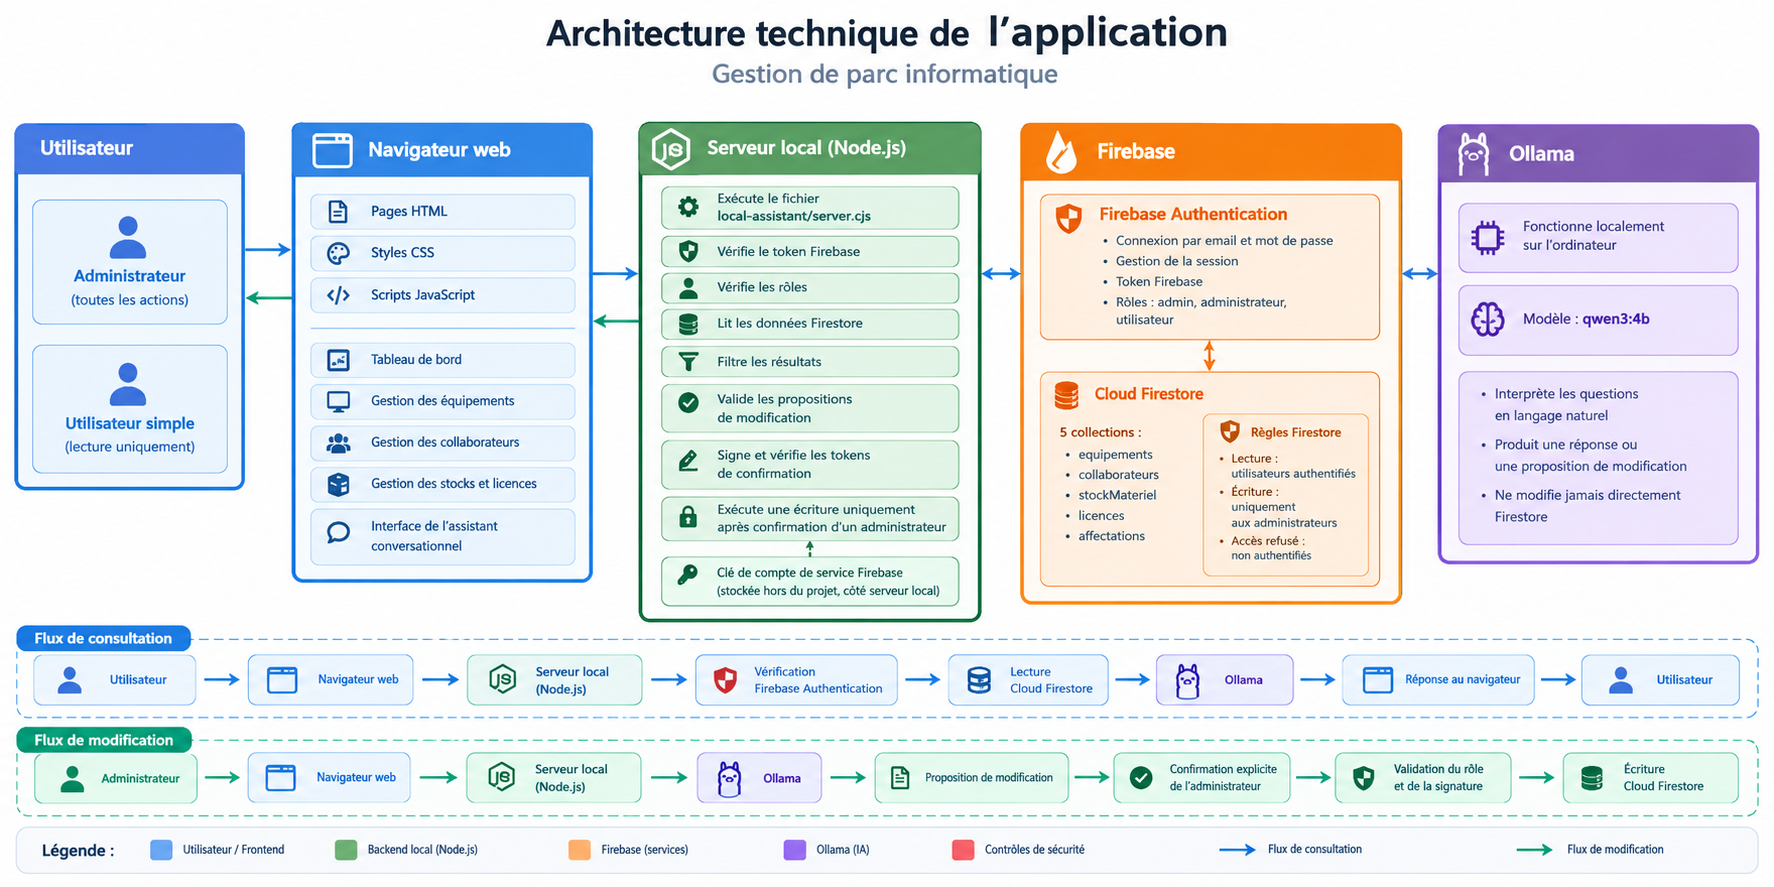
\includegraphics[width=0.90\textwidth]{architecture-systeme.png}
    \caption{Architecture générale du système}
    \label{fig:architecture-systeme}
\end{figure}

Le navigateur contient les pages HTML, les fichiers CSS et les scripts JavaScript. Il communique directement avec Firebase pour l’authentification et la consultation des données.

L’assistant conversationnel suit un autre chemin. Le navigateur envoie la demande au serveur local Node.js. Celui-ci vérifie le token Firebase, lit les données autorisées dans Firestore et communique avec Ollama pour interpréter la demande.

\section{Conception fonctionnelle}

\subsection{Acteurs du système}

Les principaux acteurs identifiés sont les suivants :

\begin{description}
    \item[Utilisateur simple :] consulte les informations du parc et interroge l’assistant en lecture seule.

    \item[Administrateur :] consulte les informations et réalise les opérations de création, modification et suppression.

    \item[Firebase Authentication :] vérifie l’identité de l’utilisateur et fournit le token contenant son rôle.

    \item[Firestore :] stocke les données du parc et applique les règles de sécurité.

    \item[Assistant Ollama :] interprète les demandes en langage naturel et produit des réponses ou des propositions de modification.
\end{description}

\subsection{Diagramme de cas d’utilisation}

\begin{figure}[htbp]
    \centering
    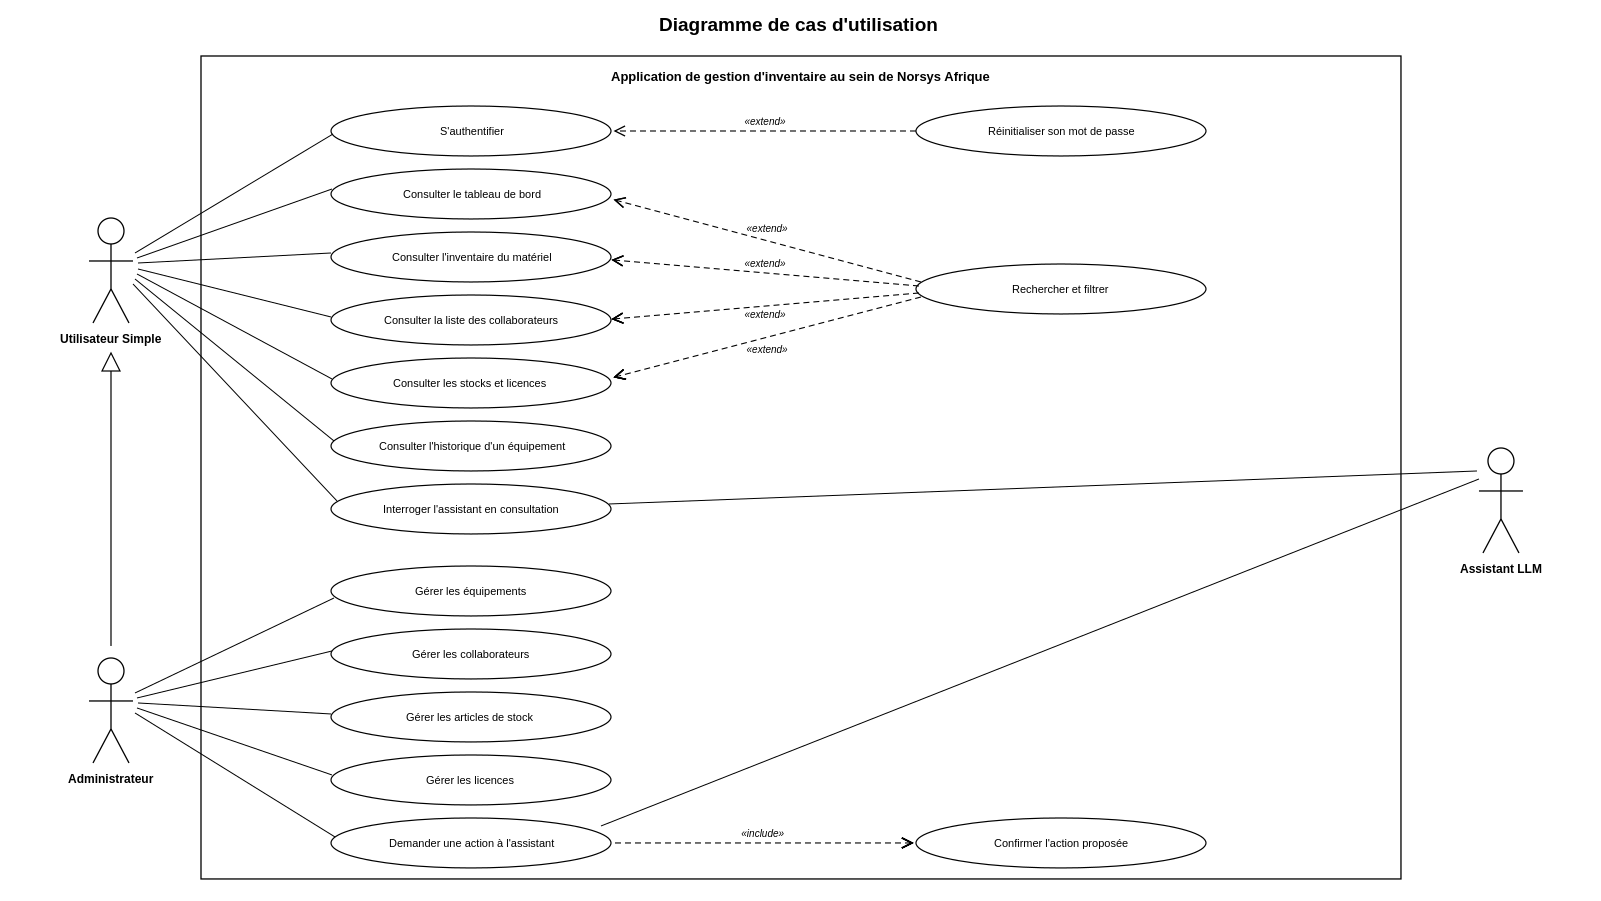
\includegraphics[width=0.95\textwidth]{diagramme/usecase_v2.png}
    \caption{Diagramme de cas d’utilisation de l’application}
    \label{fig:usecase}
\end{figure}

Les actions de gestion sont réservées à l’administrateur. Cette restriction est appliquée côté interface pour améliorer l’expérience utilisateur, mais également côté Firestore pour garantir la sécurité des données.

\section{Conception des données}

\subsection{Collections Firestore}

Le système utilise cinq collections principales :

\begin{itemize}
    \item \texttt{equipements} ;
    \item \texttt{collaborateurs} ;
    \item \texttt{stockMateriel} ;
    \item \texttt{licences} ;
    \item \texttt{affectations}.
\end{itemize}

La collection \texttt{equipements} contient une fiche par équipement physique. La collection \texttt{collaborateurs} contient les personnes susceptibles de détenir un équipement.

La collection \texttt{affectations} conserve l’historique des remises et des restitutions. Les collections \texttt{stockMateriel} et \texttt{licences} sont utilisées par la page Stocks et Licences.

\subsection{Diagramme de classes}

Le diagramme de classes représente les principales entités manipulées par l’application ainsi que leurs relations.

\begin{figure}[htbp]
    \centering
    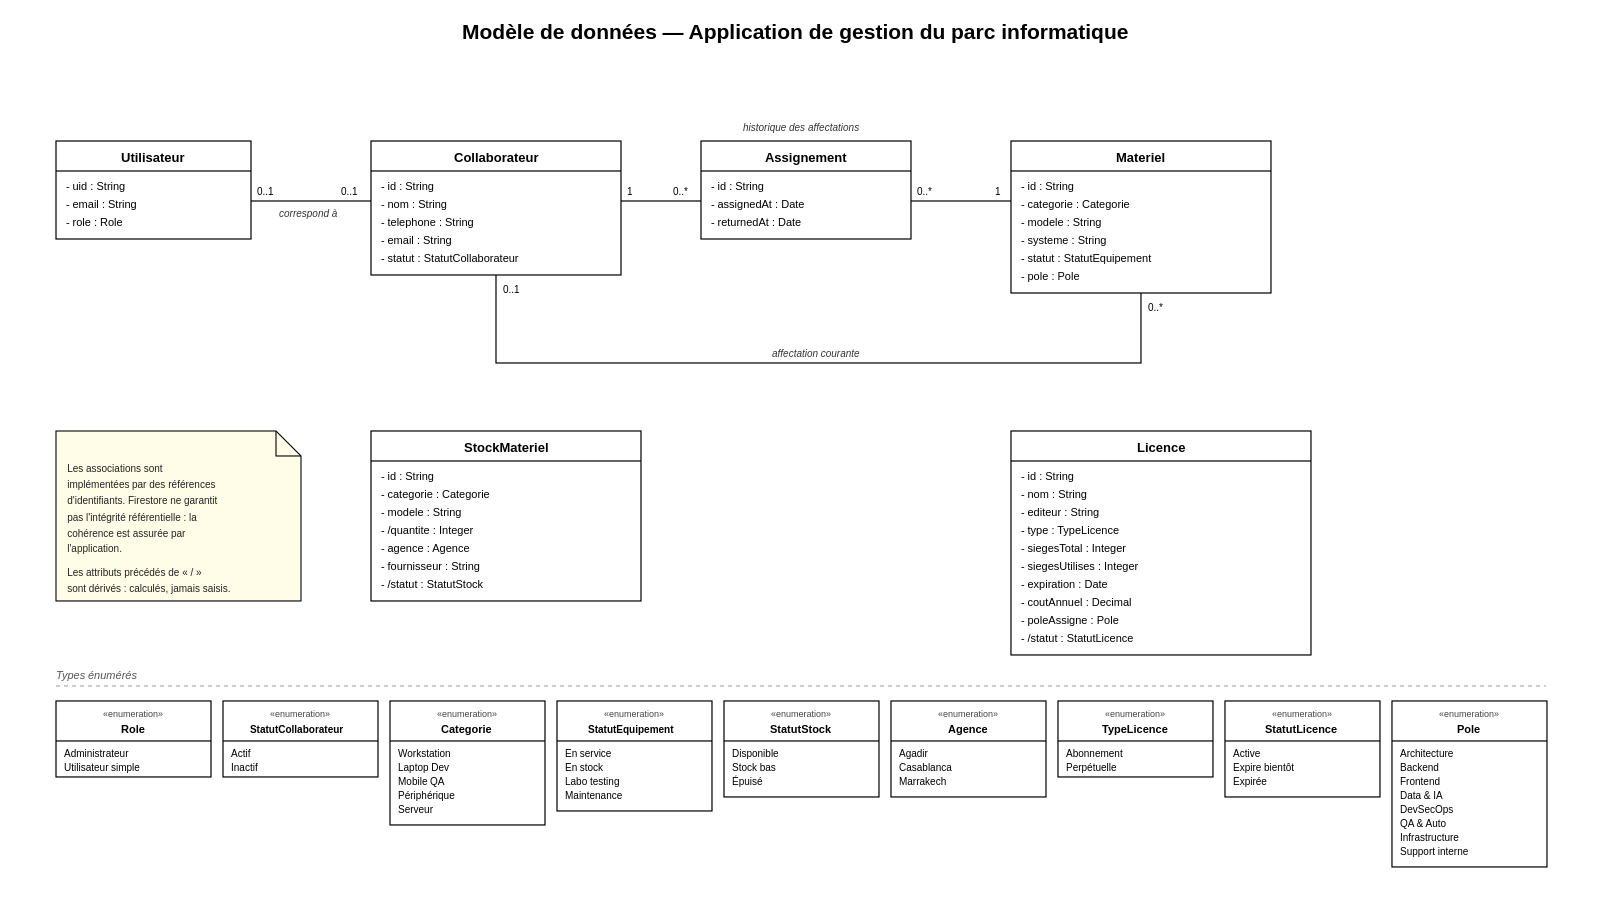
\includegraphics[width=0.95\textwidth]{diagramme/classes_modele_donnees.png}
    \caption{Diagramme de classes et modèle de données}
    \label{fig:classes}
\end{figure}

\subsection{Relations entre les classes}

Les principales relations sont les suivantes :

\begin{itemize}
    \item un collaborateur peut être associé à plusieurs équipements ;
    \item un équipement peut posséder plusieurs affectations historiques ;
    \item un collaborateur peut apparaître dans plusieurs affectations ;
    \item une affectation concerne un seul équipement ;
    \item une affectation concerne un seul collaborateur ;
    \item un équipement ne peut avoir qu’une seule affectation active.
\end{itemize}

\section{Conception des scénarios principaux}

\subsection{Scénario d’authentification}

Le scénario d’authentification commence lorsque l’utilisateur saisit son adresse email et son mot de passe.

Le déroulement est le suivant :

\begin{enumerate}
    \item l’utilisateur ouvre la page de connexion ;
    \item il saisit ses identifiants ;
    \item le navigateur transmet les informations à Firebase Authentication ;
    \item Firebase vérifie les identifiants ;
    \item Firebase retourne une session et un token ;
    \item l’application récupère le rôle de l’utilisateur ;
    \item l’utilisateur est redirigé vers le tableau de bord.
\end{enumerate}

En cas d’échec, un message est affiché et l’utilisateur reste sur la page de connexion.

Le contrôle de la session est ensuite effectué par le fichier \texttt{auth-guard.js}. Ce fichier est chargé sur les pages protégées afin d’empêcher l’accès aux utilisateurs non connectés.

\subsection{Scénario de gestion d’une affectation}

Le scénario d’affectation est réservé à l’administrateur. Une affectation active est identifiée par l’absence de date de restitution.

\subsection{Diagramme d’activité d’une affectation}

Le diagramme d’activité permet de représenter les décisions prises pendant une affectation.

\begin{figure}[htbp]
    \centering
    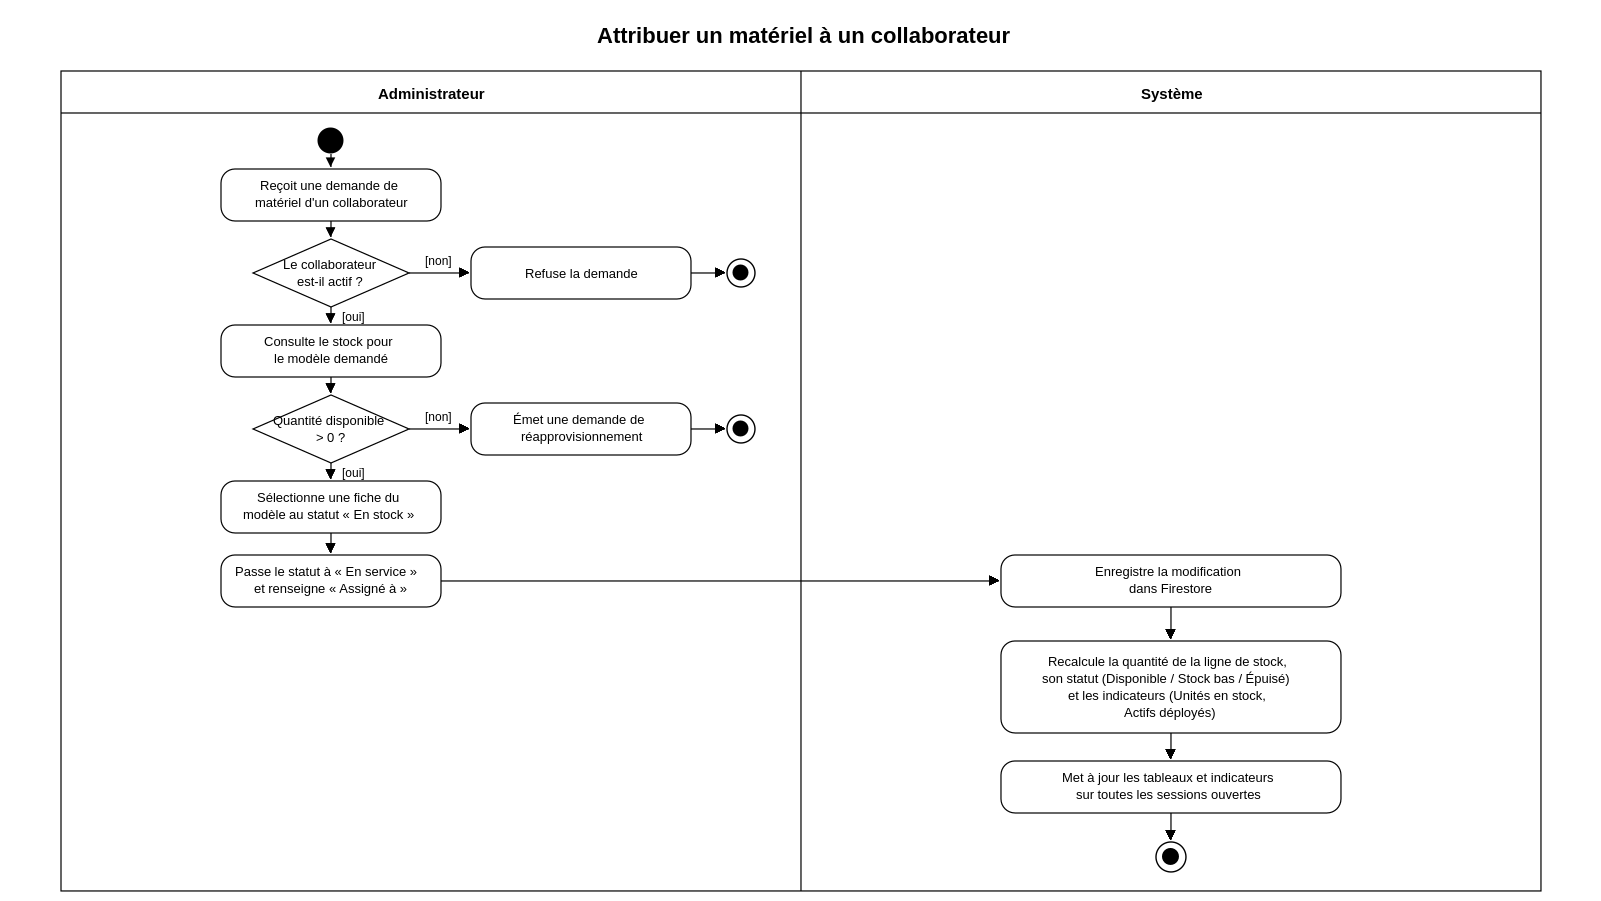
\includegraphics[width=0.90\textwidth]{diagramme/activite_attribution_staruml.png}
    \caption{Diagramme d’activité d’une affectation}
    \label{fig:activite-affectation}
\end{figure}

La validation finale vérifie qu’un équipement ne possède pas plusieurs affectations actives. Si cette condition n’est pas respectée, l’opération est refusée.

\section{Conception de l’assistant local}

\subsection{Architecture de l’assistant}

L’assistant local est composé de quatre éléments principaux :

\begin{itemize}
    \item l’interface du widget dans le navigateur ;
    \item le fichier \texttt{assistant.js} ;
    \item le serveur local \texttt{server.cjs} ;
    \item le modèle \texttt{qwen2.5:3b} exécuté par Ollama.
\end{itemize}

Le navigateur ne communique pas directement avec Ollama. Toutes les demandes passent par le serveur local Node.js.

\subsection{Séquence de consultation}

Lors d’une question de consultation, le scénario est le suivant :

\begin{enumerate}
    \item l’utilisateur saisit une question ;
    \item le navigateur récupère le token Firebase ;
    \item la question et le token sont envoyés au serveur local ;
    \item le serveur vérifie le token ;
    \item les données des collections autorisées sont lues dans Firestore ;
    \item les informations sensibles sont retirées ;
    \item Ollama interprète la demande ;
    \item les résultats sont filtrés ;
    \item Ollama rédige une réponse ;
    \item la réponse est renvoyée au navigateur.
\end{enumerate}

\begin{figure}[htbp]
    \centering
    \begin{tabular}{|p{3.2cm}|p{10.2cm}|}
        \hline
        \textbf{Étape} & \textbf{Échange ou traitement} \\
        \hline
        1. Utilisateur $\rightarrow$ navigateur & Saisie d’une question dans le widget de l’assistant. \\
        \hline
        2. Navigateur $\rightarrow$ serveur Node.js & Envoi de la question et du token Firebase. \\
        \hline
        3. Serveur Node.js $\rightarrow$ Firebase Authentication & Vérification du token et du rôle de l’utilisateur. \\
        \hline
        4. Serveur Node.js $\rightarrow$ Cloud Firestore & Lecture des données nécessaires à la consultation. \\
        \hline
        5. Serveur Node.js $\rightarrow$ Ollama & Transmission de la question pour interprétation. \\
        \hline
        6. Ollama $\rightarrow$ serveur Node.js & Retour de l’interprétation ; le serveur filtre les résultats et prépare la réponse. \\
        \hline
        7. Serveur Node.js $\rightarrow$ navigateur & Renvoi de la réponse affichée à l’utilisateur. \\
        \hline
    \end{tabular}
    \caption{Séquence de consultation avec l’assistant local}
    \label{fig:sequence-assistant}
\end{figure}

\subsection{Séquence de modification}

Lorsqu’un administrateur demande une modification, aucune écriture n’est effectuée immédiatement.

Le fonctionnement est le suivant :

\begin{enumerate}
    \item l’administrateur saisit une demande ;
    \item Ollama identifie l’action et la collection concernée ;
    \item le serveur valide la proposition ;
    \item une signature est générée ;
    \item la proposition est renvoyée au navigateur ;
    \item l’administrateur clique sur le bouton de confirmation ;
    \item le token de confirmation est vérifié ;
    \item le rôle administrateur est vérifié une nouvelle fois ;
    \item la proposition est contrôlée contre son expiration ;
    \item l’écriture est réalisée dans Firestore.
\end{enumerate}

Cette organisation sépare l’interprétation de la demande et l’exécution de l’opération. Elle permet ainsi de conserver une validation humaine avant chaque modification.

\section{Conception de la sécurité}

\subsection{Contrôle des rôles}

Le système utilise deux rôles principaux :

\begin{itemize}
    \item \texttt{admin} ou \texttt{administrateur} ;
    \item \texttt{utilisateur}.
\end{itemize}

Le rôle est contenu dans les Custom Claims du token Firebase.

Le contrôle est réalisé à plusieurs niveaux :

\begin{enumerate}
    \item l’interface masque certaines actions aux utilisateurs simples ;
    \item le serveur local vérifie le rôle avant d’accepter une proposition ;
    \item les règles Firestore refusent les écritures des utilisateurs simples.
\end{enumerate}

\subsection{Règles Firestore}

Les règles Firestore autorisent la lecture aux utilisateurs authentifiés.

Les écritures sont réservées aux administrateurs pour les collections suivantes :

\begin{itemize}
    \item \texttt{collaborateurs} ;
    \item \texttt{equipements} ;
    \item \texttt{stockMateriel} ;
    \item \texttt{licences} ;
    \item \texttt{affectations}.
\end{itemize}

Toute collection qui ne fait pas partie des collections autorisées est refusée par défaut.

\subsection{Validation des propositions}

Le fichier \texttt{assistant-core.cjs} contient la logique de validation des propositions de l’assistant.

Il contrôle notamment :

\begin{itemize}
    \item le rôle de l’utilisateur ;
    \item l’action demandée ;
    \item la collection ciblée ;
    \item l’identifiant du document ;
    \item les champs autorisés ;
    \item les statuts autorisés ;
    \item la quantité du stock ;
    \item la signature de la proposition ;
    \item l’expiration de la proposition.
\end{itemize}

Les propositions sont limitées aux actions suivantes :

\begin{itemize}
    \item \texttt{create} ;
    \item \texttt{update} ;
    \item \texttt{delete}.
\end{itemize}

La collection \texttt{affectations} n’est pas modifiable directement par l’assistant.

\section{Correspondance entre la conception et l’implémentation}

La conception UML est directement liée aux fichiers du projet.

\begin{table}[htbp]
    \centering
    \caption{Correspondance entre les éléments de conception et le code}
    \label{tab:correspondance}
    \begin{tabular}{|p{5cm}|p{8cm}|}
        \hline
        \textbf{Élément conçu} & \textbf{Élément d’implémentation} \\
        \hline
        Authentification & \texttt{auth/} et \texttt{js/auth-guard.js} \\
        \hline
        Configuration Firebase & \texttt{js/firebase-config.js} \\
        \hline
        Tableau de bord & \texttt{Dashboard/} \\
        \hline
        Gestion des équipements & \texttt{materiel/} \\
        \hline
        Gestion des collaborateurs & \texttt{collaborateur/} \\
        \hline
        Gestion du stock et des licences & \texttt{Stock-et-Licences/} \\
        \hline
        Logique des affectations & \texttt{js/assignment-lifecycle.js} \\
        \hline
        Interface de l’assistant & \texttt{js/assistant.js} \\
        \hline
        Serveur local Ollama & \texttt{local-assistant/server.cjs} \\
        \hline
        Validation des propositions & \texttt{functions/assistant-core.cjs} \\
        \hline
        Règles d’accès aux données & \texttt{firestore.rules} \\
        \hline
        Initialisation des données & \texttt{seed/} \\
        \hline
        Tests métier & \texttt{tests/} et \texttt{functions/assistant-core.test.cjs} \\
        \hline
    \end{tabular}
\end{table}

Cette correspondance montre que chaque élément important de la conception possède une responsabilité clairement identifiée dans le projet.

\section{Conclusion}

Ce chapitre a présenté la conception fonctionnelle et technique de l’application de gestion du parc informatique.

Les diagrammes UML ont permis de représenter les acteurs, les fonctionnalités, les données et les principaux scénarios d’utilisation. Le diagramme de cas d’utilisation a décrit les droits des utilisateurs et des administrateurs. Le diagramme de classes a présenté les entités principales et leurs relations. Les diagrammes de séquence et d’activité ont détaillé le fonctionnement de l’authentification, des affectations et de l’assistant local.

La conception retenue repose sur une séparation entre l’interface web, Firebase Authentication, Cloud Firestore, la logique métier partagée et le serveur local Ollama. Cette organisation facilite la compréhension, la maintenance et l’évolution du système.

Le chapitre suivant présente l’implémentation des fonctionnalités et les choix techniques réalisés lors du développement.

%================================================
% CHAPITRE 4
%================================================

\chapter{Réalisation et implémentation}

\section{Introduction}

Après avoir présenté les besoins et la conception du système, ce chapitre décrit la réalisation de l’application web de gestion du parc informatique.

L’objectif de cette étape est de transformer les modèles fonctionnels et techniques en une application opérationnelle. La réalisation concerne l’interface utilisateur, l’authentification, la gestion des données Firestore, la gestion des affectations, l’assistant local basé sur Ollama ainsi que les mécanismes de sécurité.

L’application a été développée avec des technologies web classiques afin de conserver une architecture simple et facilement maintenable. Le frontend utilise HTML, CSS et JavaScript sans framework. Firebase est utilisé pour l’authentification et le stockage des données. L’assistant conversationnel fonctionne localement à travers un serveur Node.js et le modèle \texttt{qwen2.5:3b} exécuté par Ollama.

\section{Environnement de développement}

\subsection{Technologies utilisées}

Les principales technologies utilisées sont présentées dans le tableau suivant.

\begin{table}[htbp]
    \centering
    \caption{Technologies utilisées}
    \label{tab:technologies}
    \begin{tabular}{|p{4cm}|p{8cm}|}
        \hline
        \textbf{Technologie} & \textbf{Rôle dans le projet} \\
        \hline
        HTML & Structuration des pages web. \\
        \hline
        CSS & Mise en forme et adaptation visuelle des interfaces. \\
        \hline
        JavaScript & Gestion des interactions et communication avec Firebase. \\
        \hline
        Firebase Authentication & Authentification et gestion des sessions. \\
        \hline
        Cloud Firestore & Stockage centralisé des données du parc. \\
        \hline
        Node.js & Exécution du serveur local de l'assistant. \\
        \hline
        Ollama & Exécution locale du modèle de langage. \\
        \hline
        qwen2.5:3b & Modèle utilisé pour interpréter les demandes. \\
        \hline
        GitLab & Partage et gestion des versions du code. \\
        \hline
        ClickUp & Suivi des tickets et des tâches des sprints. \\
        \hline
        Figma & Conception des maquettes des interfaces. \\
        \hline
    \end{tabular}
\end{table}

\subsection{Organisation du projet}

Le projet est organisé selon les responsabilités fonctionnelles de l’application :

\begin{itemize}
    \item \texttt{auth/} contient la page de connexion ;
    \item \texttt{Dashboard/} contient le tableau de bord ;
    \item \texttt{materiel/} contient la gestion des équipements ;
    \item \texttt{collaborateur/} contient la gestion des collaborateurs ;
    \item \texttt{Stock-et-Licences/} contient la gestion des stocks et des licences ;
    \item \texttt{js/} contient les services JavaScript partagés ;
    \item \texttt{local-assistant/} contient le serveur local Ollama ;
    \item \texttt{functions/} contient la logique de validation partagée de l’assistant ;
    \item \texttt{seed/} contient les scripts d’initialisation des données ;
    \item \texttt{tests/} contient les tests de la logique métier ;
    \item \texttt{diagramme/} contient les documents de conception et les diagrammes UML.
\end{itemize}

Cette organisation permet de séparer les pages de l’application, les services communs, la logique métier et les composants techniques.

\section{Réalisation de l’interface utilisateur}

\subsection{Structure des pages}

Chaque fonctionnalité principale possède sa propre page HTML et ses fichiers JavaScript et CSS associés.

La page de connexion se trouve dans le dossier \texttt{auth/}. Les pages fonctionnelles sont ensuite réparties selon les domaines suivants :

\begin{itemize}
    \item le tableau de bord ;
    \item les équipements ;
    \item les collaborateurs ;
    \item les stocks et les licences.
\end{itemize}

Les pages utilisent des ressources communes présentes dans le dossier \texttt{Assets/}. Ces ressources contiennent notamment des styles partagés, des logos et des éléments liés à l’affichage selon le rôle de l’utilisateur.

\subsection{Tableau de bord}

Le tableau de bord est implémenté dans le dossier \texttt{Dashboard/}. Il fournit une synthèse de l’état du parc informatique.

Les informations affichées sont calculées à partir de la collection \texttt{equipements}. Le tableau de bord présente notamment :

\begin{itemize}
    \item les équipements en service ;
    \item les équipements mobiles utilisés pour les tests ;
    \item les équipements disponibles en stock ;
    \item les équipements en maintenance ;
    \item les équipements récemment ajoutés ou modifiés.
\end{itemize}

La recherche globale permet de retrouver rapidement un équipement à partir des informations disponibles dans sa fiche.

Les indicateurs sont recalculés à chaque changement reçu de Firestore et l’inventaire est trié de la fiche la plus récemment ajoutée ou modifiée à la plus ancienne. Un administrateur peut également ajouter, modifier ou supprimer un équipement directement depuis le tableau de bord ; ces opérations sont enregistrées dans la collection \texttt{equipements}.

\subsection{Gestion des équipements}

La page de gestion des équipements est située dans le dossier \texttt{materiel/}. Elle permet de consulter et de gérer l’inventaire unitaire.

Chaque ligne affichée correspond à un équipement physique. Les principales informations présentées sont :

\begin{itemize}
    \item l’identifiant du matériel ;
    \item la catégorie ;
    \item le modèle ;
    \item le système d’exploitation ;
    \item le statut ;
    \item le collaborateur détenteur ;
    \item le pôle d’expertise ;
    \item l’agence ;
    \item le fournisseur.
\end{itemize}

Les utilisateurs authentifiés peuvent consulter les équipements. Les administrateurs peuvent également créer, modifier et supprimer les fiches.

La recherche et les filtres permettent de réduire le nombre de résultats affichés. Les critères peuvent être combinés afin d’obtenir une liste correspondant aux besoins de l’utilisateur.

Chaque ligne propose enfin une action « Affectation ». Elle ouvre une fenêtre qui affiche le détenteur actuel et l’historique complet des remises et restitutions de l’équipement. Cet historique est visible par tous les utilisateurs authentifiés ; le formulaire permettant d’affecter l’équipement à un collaborateur actif ou de le restituer n’est affiché qu’aux administrateurs.

\subsection{Gestion des collaborateurs}

La gestion des collaborateurs est implémentée dans le dossier \texttt{collaborateur/}.

La page affiche les personnes susceptibles de détenir un équipement. Elle permet notamment de consulter :

\begin{itemize}
    \item le nom du collaborateur ;
    \item son adresse email ;
    \item son numéro de téléphone ;
    \item son statut ;
    \item son rôle métier.
\end{itemize}

Les collaborateurs peuvent être recherchés et triés. Les opérations de création, de modification et de suppression sont réservées aux administrateurs.

\subsection{Gestion des stocks et des licences}

Le dossier \texttt{Stock-et-Licences/} regroupe la gestion du stock matériel et des licences.

Les articles de stock sont enregistrés dans la collection \texttt{stockMateriel}. Ils sont regroupés par catégorie, modèle, agence et fournisseur. La quantité disponible et le statut de l’article sont également suivis.

Les licences sont enregistrées dans la collection \texttt{licences}. La page permet de suivre leur nom, leur éditeur, leur type, leurs sièges, leur expiration, leur coût et le pôle concerné.

La collection \texttt{stockMateriel} est indépendante de la collection \texttt{equipements}. Les quantités du stock sont gérées directement et ne sont pas recalculées automatiquement à partir des équipements individuels.

\section{Connexion à Firebase}

\subsection{Configuration Firebase}

La configuration Firebase est centralisée dans le fichier \texttt{js/firebase-config.js}.

Ce fichier initialise l’application Firebase et exporte les services utilisés par les autres pages :

\begin{itemize}
    \item l’application Firebase ;
    \item le service d’authentification ;
    \item le service Firestore.
\end{itemize}

Un extrait simplifié de cette initialisation est présenté ci-dessous.

\begin{verbatim}
const app = initializeApp(firebaseConfig);
const auth = getAuth(app);
const db = getFirestore(app);
\end{verbatim}

Les autres fichiers JavaScript importent ensuite les objets \texttt{auth} et \texttt{db} pour accéder à Firebase.

\subsection{Authentification}

L’authentification est réalisée avec Firebase Authentication. L’utilisateur saisit son email et son mot de passe sur la page de connexion.

Après une connexion réussie, Firebase fournit un token d’identification. Ce token contient notamment les informations nécessaires à l’identification de l’utilisateur et à la récupération de son rôle.

Le fichier \texttt{auth-guard.js} est chargé sur les pages protégées. Il vérifie si une session Firebase existe.

Le fonctionnement est le suivant :

\begin{enumerate}
    \item vérifier l’état de l’authentification ;
    \item rediriger l’utilisateur vers la page de connexion s’il n’est pas connecté ;
    \item récupérer le token Firebase lorsque la session est valide ;
    \item extraire le rôle de l’utilisateur ;
    \item initialiser les fonctionnalités accessibles.
\end{enumerate}

\subsection{Gestion des rôles}

Deux profils principaux sont utilisés :

\begin{itemize}
    \item l’administrateur ;
    \item l’utilisateur simple.
\end{itemize}

Le rôle est stocké dans les Custom Claims Firebase. Il n’est donc pas saisi par l’utilisateur dans l’interface.

Après la récupération du rôle, l’application renseigne l’attribut du document HTML :

\begin{verbatim}
document.body.dataset.role = roleEffectif;
\end{verbatim}

Les fichiers CSS peuvent ensuite adapter l’affichage des boutons. Cependant, cette adaptation est uniquement visuelle. La vraie protection est assurée par les règles Firestore.

\section{Implémentation de l’accès aux données}

\subsection{Lecture des données}

Les pages utilisent le SDK JavaScript de Firebase pour lire les collections Firestore.

Les principales collections utilisées sont :

\begin{itemize}
    \item \texttt{equipements} ;
    \item \texttt{collaborateurs} ;
    \item \texttt{stockMateriel} ;
    \item \texttt{licences} ;
    \item \texttt{affectations}.
\end{itemize}

Les principales pages utilisent la fonction \texttt{onSnapshot}. Cette fonction permet de recevoir automatiquement les changements effectués dans Firestore.

Le fonctionnement est le suivant :

\begin{verbatim}
onSnapshot(collection(db, "equipements"), (snapshot) => {
    // Mise à jour de l'affichage
});
\end{verbatim}

Cette approche évite de recharger manuellement la page après chaque modification.

\subsection{Création, modification et suppression}

Les opérations d’écriture utilisent les fonctions du SDK Firestore :

\begin{itemize}
    \item \texttt{addDoc} pour créer un document ;
    \item \texttt{updateDoc} pour modifier un document ;
    \item \texttt{deleteDoc} pour supprimer un document ;
    \item \texttt{writeBatch} pour regrouper plusieurs écritures liées, comme celles d’une affectation.
\end{itemize}

Ces opérations sont accessibles dans l’interface uniquement aux administrateurs. Même si un utilisateur simple tente de contourner l’interface, les règles Firestore refusent l’écriture si son token ne contient pas un rôle administrateur.

\subsection{Règles de sécurité Firestore}

Les règles de sécurité sont définies dans le fichier \texttt{firestore.rules}.

La logique générale est la suivante :

\begin{verbatim}
Utilisateur authentifié :
    lecture autorisée

Administrateur :
    lecture et écriture autorisées

Utilisateur simple :
    lecture autorisée
    écriture refusée
\end{verbatim}

Les règles s’appliquent aux cinq collections principales. Toute autre collection est refusée par défaut.

\section{Implémentation de la gestion des affectations}

\subsection{Logique métier}

La logique de gestion des affectations est centralisée dans le fichier \texttt{js/assignment-lifecycle.js}.

Cette séparation permet de ne pas placer toutes les règles métier directement dans le code de l’interface.

La fonction de gestion d’une affectation reçoit notamment :

\begin{itemize}
    \item l’identifiant de l’équipement ;
    \item la liste des affectations existantes ;
    \item l’identifiant du nouveau collaborateur ;
    \item le nom du nouveau collaborateur ;
    \item la date.
\end{itemize}

\subsection{Détection de l’affectation active}

Une affectation est active lorsque son champ \texttt{dateRestitution} est vide ou nul.

Avant de créer une nouvelle affectation, le système vérifie le nombre d’affectations actives liées à l’équipement.

Si plusieurs affectations actives sont détectées, l’opération est refusée afin d’éviter un état incohérent.

\subsection{Création d’une nouvelle affectation}

Lorsqu’une nouvelle affectation est valide, le système :

\begin{enumerate}
    \item identifie l’affectation active existante ;
    \item ajoute la date de restitution à cette affectation ;
    \item génère l’identifiant de la nouvelle affectation ;
    \item crée la nouvelle affectation ;
    \item conserve les anciennes affectations dans l’historique ;
    \item vérifie une nouvelle fois la cohérence finale.
\end{enumerate}

Cette logique permet de conserver l’historique des détenteurs successifs d’un même équipement.

Dans la page Matériel Dev \& QA, le résultat de cette fonction est enregistré en un seul lot Firestore (\texttt{writeBatch}) contenant trois écritures : la clôture de l’ancienne affectation, la création de la nouvelle et la mise à jour de l’équipement (détenteur courant, identifiant du collaborateur et statut \texttt{En service}). Soit les trois écritures réussissent, soit aucune n’est appliquée, ce qui évite un état incohérent entre l’équipement et son historique.

La restitution suit le même principe : l’affectation active reçoit une date de restitution, et l’équipement repasse au statut \texttt{En stock} sans détenteur.

\section{Implémentation de l’assistant local}

\subsection{Architecture de l’assistant}

L’assistant local est composé de trois éléments principaux :

\begin{itemize}
    \item l’interface située dans le fichier \texttt{js/assistant.js} ;
    \item le serveur local situé dans \texttt{local-assistant/server.cjs} ;
    \item le modèle \texttt{qwen2.5:3b} exécuté par Ollama.
\end{itemize}

Le navigateur ne communique jamais directement avec Ollama. Il envoie les demandes au serveur local Node.js à l’adresse suivante :

\begin{verbatim}
http://127.0.0.1:8787/assistant
\end{verbatim}

Le modèle \texttt{qwen3:4b} avait été retenu au départ. Exécuté uniquement sur le processeur du poste, il produisait un long raisonnement interne avant chaque réponse et dépassait cinq minutes pour une simple question. Il a été remplacé par \texttt{qwen2.5:3b}, plus léger et sans phase de raisonnement, qui choisit la fonction à appeler en une vingtaine de secondes. Pendant le traitement, le widget affiche un indicateur animé indiquant que l’assistant réfléchit, puis la réponse s’écrit progressivement.

\subsection{Réception d’une demande}

Le navigateur récupère le token Firebase de l’utilisateur courant et l’envoie dans l’en-tête HTTP :

\begin{verbatim}
Authorization: Bearer <token Firebase>
\end{verbatim}

Le serveur local vérifie ensuite le token avec Firebase Admin SDK. Si le token est absent ou invalide, la demande est refusée.

\subsection{Consultation des données}

Lorsqu’une question de consultation est reçue, le serveur :

\begin{enumerate}
    \item authentifie l’utilisateur ;
    \item lit les cinq collections autorisées ;
    \item retire certains champs sensibles ;
    \item envoie la question à Ollama ;
    \item récupère la fonction demandée par le modèle ;
    \item filtre les résultats ;
    \item demande au modèle de rédiger la réponse ;
    \item renvoie la réponse au navigateur.
\end{enumerate}

Les données sensibles sont retirées avant leur transmission au modèle grâce à une fonction de nettoyage.

\subsection{Proposition d’une modification}

Une demande de modification ne provoque pas directement une écriture.

Le modèle doit produire une action structurée avec les éléments suivants :

\begin{itemize}
    \item l’action demandée ;
    \item la collection concernée ;
    \item l’identifiant du document ;
    \item les données à créer ou à modifier.
\end{itemize}

Le serveur vérifie ensuite que la proposition respecte les règles définies dans \texttt{assistant-core.cjs}.

\subsection{Confirmation d’une modification}

Après réception de la proposition, l’administrateur peut choisir de la confirmer.

Le serveur vérifie à nouveau :

\begin{itemize}
    \item l’identité de l’utilisateur ;
    \item son rôle administrateur ;
    \item la signature du token ;
    \item l’expiration de la proposition ;
    \item la collection autorisée ;
    \item les champs autorisés.
\end{itemize}

L’écriture Firestore est réalisée uniquement si toutes les vérifications réussissent.

Cette séparation entre proposition et exécution protège les données contre une mauvaise interprétation du modèle de langage.

\section{Validation des propositions}

La validation commune est implémentée dans le fichier \texttt{functions/assistant-core.cjs}.

Même si ce dossier ne contient plus de Cloud Function active, le fichier est utilisé comme bibliothèque partagée par le serveur local.

La validation porte notamment sur :

\begin{itemize}
    \item les rôles administrateurs ;
    \item les actions \texttt{create}, \texttt{update} et \texttt{delete} ;
    \item les collections qui peuvent être modifiées ;
    \item les champs autorisés pour chaque collection ;
    \item les statuts autorisés ;
    \item les quantités de stock ;
    \item les signatures cryptographiques ;
    \item la durée de validité des propositions.
\end{itemize}

La collection \texttt{affectations} n’est pas modifiable directement par l’assistant. Sa gestion passe par le parcours métier dédié aux affectations.

\section{Démarrage automatique de l’application}

\subsection{Lanceur du projet}

Le lancement du projet est automatisé par les fichiers :

\begin{itemize}
    \item \texttt{start-project.cmd} ;
    \item \texttt{start-project.ps1}.
\end{itemize}

L’utilisateur peut démarrer le projet par un double-clic sur le fichier \texttt{start-project.cmd}.

Le script PowerShell :

\begin{enumerate}
    \item vérifie la présence de la clé Firebase externe ;
    \item génère le secret de signature s’il n’existe pas ;
    \item prépare les variables d’environnement ;
    \item vérifie la disponibilité d’Ollama ;
    \item démarre le serveur local Node.js ;
    \item démarre le serveur HTTP Python ;
    \item ouvre le tableau de bord.
\end{enumerate}

Les services utilisent les ports suivants :

\begin{table}[htbp]
    \centering
    \caption{Ports utilisés par l’application}
    \label{tab:ports}
    \begin{tabular}{|p{5cm}|p{4cm}|p{4cm}|}
        \hline
        \textbf{Service} & \textbf{Adresse} & \textbf{Rôle} \\
        \hline
        Ollama & \texttt{127.0.0.1:11434} & Exécution du modèle local. \\
        \hline
        Serveur assistant & \texttt{127.0.0.1:8787} & Traitement des demandes de l’assistant. \\
        \hline
        Serveur web & \texttt{127.0.0.1:5500} & Hébergement local des pages web. \\
        \hline
    \end{tabular}
\end{table}

Si le port 5500 est déjà occupé par un autre programme, le lanceur choisit automatiquement le premier port libre entre 5501 et 5599.

\subsection{Démarrage du serveur web}

Les pages statiques sont servies par un serveur HTTP local Python.

L’adresse principale de l’application est :

\begin{verbatim}
http://127.0.0.1:5500/Dashboard/index.html
\end{verbatim}

Le serveur HTTP permet au navigateur de charger correctement les modules JavaScript et les ressources de l’application.

\section{Initialisation des données}

\subsection{Initialisation de Firestore}

Le fichier \texttt{seed/firestore-seed.mjs} contient les données initiales du projet.

Il permet d’insérer les données de départ dans les collections suivantes :

\begin{itemize}
    \item \texttt{collaborateurs} ;
    \item \texttt{equipements} ;
    \item \texttt{stockMateriel} ;
    \item \texttt{licences} ;
    \item \texttt{affectations}.
\end{itemize}

La clé de compte de service est chargée à partir de la variable :

\begin{verbatim}
GOOGLE_APPLICATION_CREDENTIALS
\end{verbatim}

Elle est conservée à l’extérieur du projet afin de ne pas être exposée dans le dépôt.

\subsection{Initialisation des rôles}

Le fichier \texttt{seed/setup-roles.mjs} permet de préparer les comptes Firebase et leurs rôles.

Les rôles sont stockés dans les Custom Claims Firebase. Cette information est ensuite utilisée par :

\begin{itemize}
    \item le garde d’authentification ;
    \item l’interface utilisateur ;
    \item le serveur local ;
    \item les règles Firestore.
\end{itemize}

\section{Méthodologie d’implémentation}

Le développement a été réalisé selon une démarche Agile Scrum organisée en trois sprints.

Les tâches étaient décrites sous forme de tickets dans ClickUp. Chaque ticket correspondait à une fonctionnalité, une correction, une amélioration ou une tâche de documentation.

Les maquettes des pages ont été préparées avec Figma avant leur implémentation en HTML et CSS.

Le code était partagé et versionné avec GitLab. Cette organisation a permis de conserver l’historique des modifications et de synchroniser le travail entre les membres de l’équipe.

Les sprints ont permis de progresser de manière incrémentale :

\begin{description}
    \item[Premier sprint :] analyse des besoins, définition du périmètre et préparation des maquettes.

    \item[Deuxième sprint :] développement des pages principales, connexion à Firebase et gestion des premières collections.

    \item[Troisième sprint :] ajout des affectations, amélioration de la sécurité, intégration de l’assistant local, tests et documentation.
\end{description}

\section{Conclusion}

Ce chapitre a présenté la réalisation et l’implémentation de l’application web de gestion du parc informatique.

L’interface a été développée en HTML, CSS et JavaScript. Firebase Authentication permet de gérer les utilisateurs et leurs rôles, tandis que Cloud Firestore centralise les données du parc.

Les principales pages de l’application permettent de gérer les équipements, les collaborateurs, les stocks, les licences et les affectations. La logique des affectations est séparée dans un module métier dédié afin de garantir la cohérence de l’historique.

L’assistant local repose sur un serveur Node.js et le modèle \texttt{qwen2.5:3b} exécuté avec Ollama. Les demandes de modification sont contrôlées, signées et soumises à une confirmation explicite avant toute écriture.

Enfin, l’utilisation de Figma, ClickUp, GitLab et de la méthode Agile Scrum a permis d’organiser le développement et de faciliter le suivi des différentes étapes de réalisation. Le chapitre suivant présente les tests effectués et les résultats obtenus.

%================================================
% CHAPITRE 5
%================================================

\chapter{Tests et évaluation de l’application}

\section{Introduction}

Après avoir présenté la réalisation et l’implémentation de l’application, ce chapitre est consacré aux tests et à l’évaluation de la solution développée.

Les tests ont pour objectif de vérifier que les fonctionnalités principales répondent aux besoins identifiés et que les règles de sécurité sont correctement appliquées. Une attention particulière a été accordée à la gestion des affectations, au contrôle des rôles et au fonctionnement des propositions de modification générées par l’assistant local.

La stratégie de validation repose sur plusieurs niveaux de tests :

\begin{itemize}
    \item les tests unitaires de la logique métier ;
    \item les tests de validation des propositions de l’assistant ;
    \item les tests de contrôle des rôles et des droits d’accès ;
    \item les tests fonctionnels des principales pages ;
    \item les tests de démarrage et de communication entre les composants.
\end{itemize}

\section{Stratégie de test}

Les tests ont été réalisés à partir des règles métier et des fonctionnalités définies dans les chapitres précédents.

Chaque fonctionnalité importante a été associée à un comportement attendu. Le résultat obtenu a ensuite été comparé à ce comportement afin de déterminer si le test était réussi ou non.

La stratégie adoptée consiste à tester progressivement :

\begin{enumerate}
    \item les fonctions métier indépendantes de l’interface ;
    \item les contrôles de sécurité ;
    \item les opérations de lecture et d’écriture ;
    \item les interactions entre le navigateur, Firebase et le serveur local ;
    \item les scénarios complets d’utilisation.
\end{enumerate}

Cette organisation permet de détecter les erreurs à différents niveaux et de faciliter leur correction.

\section{Environnement de test}

Les tests ont été réalisés dans l’environnement local du projet.

Les principaux composants utilisés sont :

\begin{table}[htbp]
    \centering
    \caption{Environnement de test}
    \label{tab:env-test}
    \begin{tabular}{|p{5cm}|p{8cm}|}
        \hline
        \textbf{Composant} & \textbf{Utilisation} \\
        \hline
        Node.js & Exécution des tests JavaScript et du serveur local. \\
        \hline
        Firebase Authentication & Vérification des sessions et des rôles. \\
        \hline
        Cloud Firestore & Lecture et écriture des données. \\
        \hline
        Ollama & Exécution locale du modèle de langage. \\
        \hline
        qwen2.5:3b & Interprétation des demandes adressées à l’assistant. \\
        \hline
        Navigateur web & Vérification du comportement des pages. \\
        \hline
        Python HTTP Server & Mise à disposition locale des fichiers web. \\
        \hline
    \end{tabular}
\end{table}

Le lancement de l’environnement est simplifié par le fichier \texttt{start-project.cmd}. Celui-ci démarre les services nécessaires et ouvre le tableau de bord dans le navigateur.

Les services utilisés pendant les tests sont :

\begin{itemize}
    \item Ollama sur le port \texttt{11434} ;
    \item le serveur assistant sur le port \texttt{8787} ;
    \item le serveur web sur le port \texttt{5500}.
\end{itemize}

\section{Tests unitaires de la gestion des affectations}

\subsection{Objectif des tests}

La gestion des affectations constitue une fonctionnalité importante du projet. Elle doit garantir la cohérence entre l’équipement, le collaborateur et l’historique des remises et des restitutions.

La logique métier est regroupée dans le fichier \texttt{js/assignment-lifecycle.js}. Les tests associés se trouvent dans le fichier \texttt{tests/assignment-lifecycle.test.mjs}.

\subsection{Clôture d’une affectation existante}

Le premier test vérifie qu’une ancienne affectation active est correctement clôturée lorsqu’un équipement est affecté à un nouveau collaborateur.

Le comportement attendu est le suivant :

\begin{enumerate}
    \item identifier l’affectation active ;
    \item renseigner sa date de restitution ;
    \item créer une nouvelle affectation ;
    \item renseigner la date de remise de la nouvelle affectation ;
    \item conserver l’historique précédent.
\end{enumerate}

Le test vérifie également que la nouvelle affectation contient les identifiants corrects de l’équipement et du collaborateur.

Le résultat obtenu est conforme au comportement attendu.

\subsection{Compatibilité des noms de champs}

Les données historiques du projet utilisent parfois des noms de champs français et anglais. Par exemple :

\begin{itemize}
    \item \texttt{equipmentId} et \texttt{equipementId} ;
    \item \texttt{collaboratorId} et \texttt{collaborateurId} ;
    \item \texttt{collaboratorNom} et \texttt{collaborateurNom}.
\end{itemize}

Un test spécifique vérifie que la logique d’affectation accepte les noms de champs français utilisés dans les documents Firestore.

Ce test est important car il permet de maintenir la compatibilité avec les données déjà présentes dans la base.

Le test est réussi.

\subsection{Refus de plusieurs affectations actives}

Une règle métier essentielle impose qu’un équipement ne possède jamais plusieurs affectations actives.

Le test fournit deux affectations actives pour le même équipement. La fonction de validation doit alors lever une erreur.

Le résultat attendu est obtenu : l’état incohérent est refusé.

\begin{table}[htbp]
    \centering
    \caption{Tests de la logique des affectations}
    \label{tab:tests-affectations}
    \begin{tabular}{|p{7cm}|p{3cm}|p{3cm}|}
        \hline
        \textbf{Test} & \textbf{Résultat attendu} & \textbf{Résultat obtenu} \\
        \hline
        Clôture de l’ancienne affectation & Succès & Réussi \\
        \hline
        Création de la nouvelle affectation & Succès & Réussi \\
        \hline
        Compatibilité des noms de champs & Acceptation & Réussi \\
        \hline
        Refus de plusieurs affectations actives & Erreur & Réussi \\
        \hline
    \end{tabular}
\end{table}

\section{Tests de validation de l’assistant}

\subsection{Objectif des tests}

L’assistant local peut produire des propositions de création, de modification ou de suppression. Ces propositions doivent être vérifiées avant toute exécution.

La logique de validation est regroupée dans le fichier \texttt{functions/assistant-core.cjs}. Les tests associés sont présents dans le fichier \texttt{functions/assistant-core.test.cjs}.

\subsection{Validation des rôles}

Le premier test vérifie que les rôles administrateurs reconnus par le système sont correctement identifiés.

Les rôles suivants sont acceptés :

\begin{itemize}
    \item \texttt{admin} ;
    \item \texttt{administrateur}.
\end{itemize}

Le rôle \texttt{utilisateur} ne doit pas être considéré comme administrateur.

Le test confirme que les utilisateurs simples ne peuvent pas effectuer d’opérations réservées aux administrateurs.

\subsection{Signature des propositions}

Lorsqu’une proposition est créée, elle est signée avec un secret.

Le test vérifie les opérations suivantes :

\begin{enumerate}
    \item créer une proposition valide ;
    \item générer une signature ;
    \item vérifier la signature ;
    \item retrouver la proposition d’origine ;
    \item refuser une proposition dont le token a été modifié.
\end{enumerate}

Le test confirme qu’une modification du token entraîne le refus de la confirmation.

\subsection{Validation des champs autorisés}

Les propositions de modification ne peuvent pas contenir n’importe quel champ.

Le test vérifie que :

\begin{itemize}
    \item les champs autorisés sont acceptés ;
    \item les champs sensibles sont refusés ;
    \item les collections non modifiables sont refusées ;
    \item les propositions vides sont refusées.
\end{itemize}

Par exemple, une tentative de modification contenant un champ sensible tel que \texttt{rib} est rejetée.

La collection \texttt{affectations} ne peut pas être modifiée directement par l’assistant. Elle doit être gérée par le processus métier prévu dans l’application.

\subsection{Résultats des tests de l’assistant}

\begin{table}[htbp]
    \centering
    \caption{Tests du cœur de validation de l’assistant}
    \label{tab:tests-assistant}
    \begin{tabular}{|p{7cm}|p{3cm}|p{3cm}|}
        \hline
        \textbf{Test} & \textbf{Résultat attendu} & \textbf{Résultat obtenu} \\
        \hline
        Reconnaissance d’un rôle administrateur & Administrateur reconnu & Réussi \\
        \hline
        Refus d’un utilisateur simple & Accès refusé & Réussi \\
        \hline
        Signature d’une proposition & Token valide & Réussi \\
        \hline
        Modification d’un token signé & Token refusé & Réussi \\
        \hline
        Refus d’un champ sensible & Proposition refusée & Réussi \\
        \hline
        Refus de la modification d’une affectation & Proposition refusée & Réussi \\
        \hline
    \end{tabular}
\end{table}

\section{Tests de sécurité}

\subsection{Accès sans authentification}

Un utilisateur non connecté ne doit pas pouvoir accéder aux pages métier.

Le fichier \texttt{auth-guard.js} surveille l’état de la session Firebase. Lorsque la session est absente, l’utilisateur est redirigé vers la page de connexion.

Le comportement attendu est le suivant :

\begin{verbatim}
Utilisateur non authentifié
        |
        v
Tentative d'accès à une page protégée
        |
        v
Redirection vers la page de connexion
\end{verbatim}

Ce comportement permet d’empêcher l’accès direct aux pages de l’application.

\subsection{Accès en lecture pour un utilisateur simple}

Un utilisateur simple authentifié peut consulter les données du parc.

Il peut accéder :

\begin{itemize}
    \item au tableau de bord ;
    \item aux équipements ;
    \item aux collaborateurs ;
    \item aux stocks ;
    \item aux licences ;
    \item à l’historique des affectations.
\end{itemize}

Les lectures sont autorisées par les règles Firestore lorsque le token Firebase est présent.

\subsection{Refus des écritures pour un utilisateur simple}

Un utilisateur simple ne doit pas pouvoir :

\begin{itemize}
    \item créer un équipement ;
    \item modifier un équipement ;
    \item supprimer un équipement ;
    \item modifier un collaborateur ;
    \item modifier un article de stock ;
    \item modifier une licence ;
    \item confirmer une proposition de modification.
\end{itemize}

Même si l’utilisateur tente de contourner les éléments de l’interface, les règles Firestore doivent refuser l’opération d’écriture.

\subsection{Accès administrateur}

Un administrateur authentifié peut effectuer les opérations d’écriture autorisées sur les collections du projet.

Son rôle est vérifié :

\begin{itemize}
    \item dans l’interface ;
    \item dans le serveur local de l’assistant ;
    \item dans les règles de sécurité Firestore.
\end{itemize}

La vérification à plusieurs niveaux permet de réduire les risques liés à une modification non autorisée.

\section{Tests fonctionnels des pages}

\subsection{Test de la page de connexion}

Le test de la page de connexion vérifie les scénarios suivants :

\begin{table}[htbp]
    \centering
    \caption{Tests fonctionnels de la connexion}
    \label{tab:tests-connexion}
    \begin{tabular}{|p{6cm}|p{4cm}|p{3cm}|}
        \hline
        \textbf{Scénario} & \textbf{Comportement attendu} & \textbf{État} \\
        \hline
        Identifiants valides & Accès au tableau de bord & Validé \\
        \hline
        Mot de passe incorrect & Message d’erreur & Validé \\
        \hline
        Email inexistant & Connexion refusée & Validé \\
        \hline
        Accès à une page sans session & Redirection vers connexion & Validé \\
        \hline
        Déconnexion & Retour vers connexion & Validé \\
        \hline
    \end{tabular}
\end{table}

\subsection{Test du tableau de bord}

Le tableau de bord est vérifié à partir des données présentes dans la collection \texttt{equipements}.

Les contrôles portent sur :

\begin{itemize}
    \item le chargement des équipements ;
    \item le calcul des indicateurs ;
    \item l’affichage des équipements récents ;
    \item la recherche globale ;
    \item l’actualisation après une modification Firestore.
\end{itemize}

Le tableau de bord doit présenter des informations cohérentes avec les données disponibles dans Firestore.

\subsection{Test de la page des équipements}

Les fonctionnalités testées sont :

\begin{itemize}
    \item affichage des équipements ;
    \item recherche par modèle ou identifiant ;
    \item filtrage par catégorie ;
    \item filtrage par statut ;
    \item création d’un équipement par un administrateur ;
    \item modification d’un équipement par un administrateur ;
    \item suppression d’un équipement par un administrateur ;
    \item affichage de l’historique des affectations d’un équipement ;
    \item affectation d’un équipement à un nouveau collaborateur, avec clôture de l’affectation précédente ;
    \item restitution d’un équipement ;
    \item refus des écritures pour un utilisateur simple.
\end{itemize}

\subsection{Test de la page des collaborateurs}

Les scénarios vérifiés sont :

\begin{itemize}
    \item affichage de la liste des collaborateurs ;
    \item recherche d’un collaborateur ;
    \item tri de la liste ;
    \item création d’une fiche ;
    \item modification d’une fiche ;
    \item suppression d’une fiche ;
    \item contrôle des droits selon le rôle.
\end{itemize}

\subsection{Test de la page Stocks et Licences}

Les contrôles portent sur :

\begin{itemize}
    \item l’affichage des articles de stock ;
    \item la modification de la quantité ;
    \item l’affichage du statut du stock ;
    \item l’affichage des licences ;
    \item l’ajout d’une licence ;
    \item la modification d’une licence ;
    \item la suppression d’une licence ;
    \item la limitation des écritures aux administrateurs.
\end{itemize}

\section{Tests de l’assistant local}

\subsection{Test de démarrage}

Le démarrage automatique est réalisé avec le fichier \texttt{start-project.cmd}.

Le lanceur vérifie la présence des services suivants :

\begin{itemize}
    \item Ollama ;
    \item le modèle \texttt{qwen2.5:3b} ;
    \item le serveur assistant Node.js ;
    \item le serveur web local ;
    \item la clé Firebase externe.
\end{itemize}

Les ports utilisés sont :

\begin{table}[htbp]
    \centering
    \caption{Vérification des services locaux}
    \label{tab:services-locaux}
    \begin{tabular}{|p{5cm}|p{4cm}|p{4cm}|}
        \hline
        \textbf{Service} & \textbf{Port} & \textbf{Résultat attendu} \\
        \hline
        Ollama & 11434 & Service disponible \\
        \hline
        Serveur assistant & 8787 & Route \texttt{/assistant} disponible \\
        \hline
        Serveur web & 5500 & Dashboard accessible \\
        \hline
    \end{tabular}
\end{table}

\subsection{Test d’une question de consultation}

Un utilisateur authentifié peut poser une question à l’assistant.

Un exemple de scénario est :

\begin{verbatim}
Utilisateur :
Quels équipements sont actuellement en stock ?
\end{verbatim}

Le système doit :

\begin{enumerate}
    \item vérifier la session Firebase ;
    \item envoyer la question au serveur local ;
    \item lire les données Firestore ;
    \item filtrer les équipements correspondants ;
    \item demander à Ollama de rédiger une réponse ;
    \item afficher la réponse dans le widget assistant.
\end{enumerate}

Aucune écriture ne doit être effectuée pendant une consultation.

\subsection{Test d’une demande de modification}

Un administrateur peut demander une modification à l’assistant.

Un exemple de scénario est :

\begin{verbatim}
Administrateur :
Modifier le statut de l'équipement NRS-LPT-101 en Maintenance.
\end{verbatim}

Le système doit générer une proposition contenant :

\begin{itemize}
    \item l’action \texttt{update} ;
    \item la collection \texttt{equipements} ;
    \item l’identifiant du document ;
    \item la donnée à modifier.
\end{itemize}

La modification ne doit pas être exécutée avant la confirmation de l’administrateur.

\subsection{Test d’une confirmation}

Lorsqu’une proposition est affichée, l’administrateur peut cliquer sur le bouton de confirmation.

Le serveur doit vérifier :

\begin{enumerate}
    \item le token Firebase ;
    \item le rôle administrateur ;
    \item la signature de la proposition ;
    \item l’identité de l’utilisateur ;
    \item la date d’expiration ;
    \item les données de la proposition.
\end{enumerate}

Si tous les contrôles réussissent, l’écriture est effectuée dans Firestore. Dans le cas contraire, la confirmation est refusée.

\section{Résultats globaux}

Les tests automatisés réalisés sur le projet ont permis de valider les règles principales de la logique métier.

Les résultats obtenus sont les suivants :

\begin{table}[htbp]
    \centering
    \caption{Résultats globaux des tests automatisés}
    \label{tab:resultats-globaux}
    \begin{tabular}{|p{7cm}|p{3cm}|p{3cm}|}
        \hline
        \textbf{Domaine} & \textbf{Tests} & \textbf{Résultat} \\
        \hline
        Cycle de vie des affectations & 3 & Réussis \\
        \hline
        Rôles et autorisations de l’assistant & 1 & Réussi \\
        \hline
        Signature des propositions & 1 & Réussi \\
        \hline
        Validation des champs sensibles & 1 & Réussi \\
        \hline
        \textbf{Total} & \textbf{6} & \textbf{Réussis} \\
        \hline
    \end{tabular}
\end{table}

Les tests ont confirmé les points suivants :

\begin{itemize}
    \item une ancienne affectation peut être clôturée correctement ;
    \item une nouvelle affectation est créée avec les informations attendues ;
    \item plusieurs affectations actives pour un même équipement sont refusées ;
    \item les rôles administrateurs sont correctement reconnus ;
    \item les tokens de confirmation sont vérifiés ;
    \item les tokens modifiés sont refusés ;
    \item les champs sensibles ne peuvent pas être ajoutés dans une proposition ;
    \item les collections non autorisées ne peuvent pas être modifiées par l’assistant.
\end{itemize}

\section{Limites identifiées}

Même si les fonctionnalités principales sont opérationnelles, certaines limites subsistent dans la version actuelle.

\subsection{Dépendance au poste local}

L’assistant dépend de la présence d’Ollama et du modèle \texttt{qwen2.5:3b} sur le poste utilisé.

Le serveur local doit être démarré pour utiliser l’assistant. Cette architecture convient à une utilisation locale, mais elle ne permet pas encore un accès distant depuis plusieurs ordinateurs.

Les performances dépendent également du matériel. Sans carte graphique exploitable par Ollama, le modèle s’exécute uniquement sur le processeur : une réponse complète, qui nécessite deux appels au modèle, demande environ vingt à quarante secondes. Un petit modèle peut aussi commettre des erreurs d’interprétation, notamment sur les questions de comptage ; c’est l’une des raisons pour lesquelles les modifications restent soumises à une confirmation humaine.

\subsection{Gestion indépendante du stock}

La collection \texttt{stockMateriel} est gérée séparément de la collection \texttt{equipements}. Une modification d’un équipement ne recalcule donc pas automatiquement les quantités du stock.

Cette limite doit être prise en compte lors de l’interprétation des données.

\subsection{Couverture des tests}

Les tests automatisés couvrent principalement la logique métier des affectations et la validation de l’assistant.

Des tests supplémentaires pourraient être ajoutés pour :

\begin{itemize}
    \item les règles Firestore dans un environnement de test ;
    \item les scénarios complets dans un navigateur ;
    \item les erreurs de communication avec Ollama ;
    \item les performances lorsque le nombre de documents augmente ;
    \item la cohérence entre l’équipement et son affectation courante.
\end{itemize}

\subsection{Dépendance à la qualité des données}

La qualité des résultats dépend également de la cohérence des données présentes dans Firestore. Des informations incomplètes ou contradictoires peuvent influencer l’affichage des pages et les réponses de l’assistant.

\section{Conclusion}

Ce chapitre a présenté la stratégie de test et l’évaluation de l’application de gestion du parc informatique.

Les tests de la logique des affectations ont confirmé la bonne gestion des remises, des restitutions et de l’historique. Les tests du cœur de validation de l’assistant ont confirmé le contrôle des rôles, des champs autorisés et des signatures.

Les tests fonctionnels permettent également de vérifier le comportement des principales pages : connexion, tableau de bord, équipements, collaborateurs, stocks, licences et assistant local.

Les résultats obtenus montrent que les règles métier principales sont respectées et que les opérations sensibles sont protégées par plusieurs niveaux de contrôle. Certaines limites subsistent, notamment la dépendance au poste local pour Ollama, la gestion indépendante du stock et la couverture encore limitée des tests d’intégration.

Ces résultats permettent de conclure que la solution répond aux besoins principaux définis pour la première version du projet, tout en laissant des possibilités d’amélioration pour les évolutions futures.

%================================================
% CONCLUSION GENERALE
%================================================

\newpage
\chapter*{Conclusion générale}
\addcontentsline{toc}{chapter}{Conclusion générale}

Ce projet de stage d’été a permis de concevoir et de développer une application web de gestion du parc informatique répondant à un besoin concret de gestion, de suivi et de sécurisation des ressources technologiques.

L’outil mis en place centralise les informations relatives aux équipements, aux collaborateurs, aux affectations, aux stocks et aux licences, ce qui facilite l’exploitation et la traçabilité des données. L’architecture retenue, basée sur des technologies web légères et des services cloud gérés, permet une mise en œuvre rapide tout en assurant une bonne séparation des rôles et une protection des opérations sensibles.

L’intégration d’un assistant intelligent local constitue un atout supplémentaire, car elle facilite l’accès aux données et la génération de propositions d’actions en langage naturel. Toutefois, la validation humaine reste nécessaire pour garantir la fiabilité des opérations et limiter les risques liés aux modifications non contrôlées.

En somme, ce travail a permis de valider la faisabilité d’une solution de gestion du parc informatique adaptée à un environnement professionnel. Il constitue une base solide pour des évolutions futures, notamment l’ajout de nouvelles fonctionnalités, l’amélioration de l’automatisation et la mise en place d’un système encore plus complet et plus performant.

%================================================
% BIBLIOGRAPHIE
%================================================

\newpage

\begin{thebibliography}{9}
    \bibitem{firebase} Google, \emph{Firebase Documentation}, 2026.
    \bibitem{firestore} Google, \emph{Cloud Firestore Documentation}, 2026.
    \bibitem{html} W3C, \emph{HTML Living Standard}, 2026.
    \bibitem{ollama} Ollama, \emph{Documentation officielle du moteur d’exécution local de modèles IA}, 2026.
    \bibitem{uml} Jacobson, I., Booch, G., Rumbaugh, J., \emph{The Unified Software Development Process}, Addison-Wesley, 1999.
\end{thebibliography}

%================================================
% ANNEXES
%================================================

\newpage
\appendix
\chapter*{Annexes}
\addcontentsline{toc}{chapter}{Annexes}
\markboth{Annexes}{Annexes}

\section*{Annexe A. Exemples d’interfaces principales}
\phantomsection
\addcontentsline{toc}{section}{Annexe A. Exemples d’interfaces principales}

\noindent Le présent rapport s’inscrit dans le cadre d’un stage d’été réalisé au sein de Norsys Afrique, dans le cadre de la formation d’ingénieur à l’ENSIAS. L’application développée a été conçue pour répondre à un besoin réel de gestion du parc informatique et pour démontrer la capacité à transformer un cahier des charges fonctionnel en un outil exploitable, structuré et sécurisé.

\vspace{0.5cm}
\noindent Les éléments exposés dans cette annexe illustrent l’architecture générale du système, les principaux écrans et les flux de gestion des équipements, des affectations, des stocks et des licences. Ils complètent la description technique fournie dans le corps du rapport et mettent en évidence l’orientation pratique du projet.

\section*{Annexe B. Extrait de code de l’interface principale}
\phantomsection
\addcontentsline{toc}{section}{Annexe B. Extrait de code de l’interface principale}

\noindent L’extrait HTML suivant présente la structure des indicateurs et du tableau d’inventaire visibles sur le tableau de bord. Les styles CSS ont été omis afin de faciliter la lecture.

\begin{minted}[fontsize=\small,breaklines,linenos,frame=single]{html}
<section class="page-title">
    <h1>Supervision du Parc Informatique</h1>
    <p>Vue d'ensemble des équipements d'agence - Agadir</p>
</section>

<section class="stats-grid">
    <div class="stat-card">
        <div class="stat-info">
            <h3>Actifs déployés</h3>
            <span class="stat-number">0</span> <!-- calculé en JS -->
        </div>
    </div>
    <div class="stat-card">
        <div class="stat-info">
            <h3>Flotte mobile (QA)</h3>
            <span class="stat-number">0</span>
        </div>
    </div>
    <div class="stat-card">
        <div class="stat-info">
            <h3>En stock / préparation</h3>
            <span class="stat-number">0</span>
        </div>
    </div>
    <div class="stat-card">
        <div class="stat-info">
            <h3>Maintenance requise</h3>
            <span class="stat-number">0</span>
        </div>
    </div>
</section>

<section class="inventory-section">
    <div class="inventory-header">
        <h2>Inventaire Récent</h2>
        <select class="category-filter filter-select">
            <option value="all">Toutes les catégories</option>
        </select>
        <button type="button" class="btn-primary admin-only">
            Nouvel Équipement
        </button>
    </div>
    <table class="data-table inventory-table">
        <thead>
            <tr>
                <th>ID matériel</th>
                <th>Catégorie</th>
                <th>Modèle</th>
                <th>Système / OS</th>
                <th>Statut</th>
                <th>Assigné à</th>
                <th>Pôle d'expertise</th>
            </tr>
        </thead>
        <tbody id="inventory-body"></tbody>
    </table>
</section>
\end{minted}

\noindent Les lignes du tableau sont alimentées en temps réel depuis la collection \texttt{equipements} de Cloud Firestore. L’extrait JavaScript ci-dessous transforme les documents reçus puis actualise les indicateurs et l’inventaire.

\begin{minted}[fontsize=\small,breaklines,linenos,frame=single]{javascript}
onSnapshot(collection(db, "equipements"), (snapshot) => {
    equipements = snapshot.docs.map((doc) => {
        const data = doc.data();
        return {
            docId: doc.id,
            id: data.idMateriel || data.id || doc.id,
            categorie: data.categorie || "-",
            modele: data.modele || "-",
            os: data.systemeOS || data.os || "-",
            statut: data.statut || "En stock",
            assigneA: data.assigneA || "-",
            pole: data.poleExpertise || data.pole || "-",
        };
    });
    refreshAll();
});
\end{minted}

\section*{Annexe C. Schéma d’architecture du système}
\phantomsection
\addcontentsline{toc}{section}{Annexe C. Schéma d’architecture du système}

\noindent La figure suivante présente les principaux composants de l’application et leurs échanges : l’utilisateur accède au frontend dans son navigateur, lequel communique avec Firebase pour l’authentification et les données. Pour les requêtes de l’assistant, le serveur local Node.js vérifie l’identité et les autorisations, puis sollicite Ollama. Une modification n’est enregistrée dans Firestore qu’après validation et confirmation explicite d’un administrateur.

\begin{figure}[htbp]
    \centering
    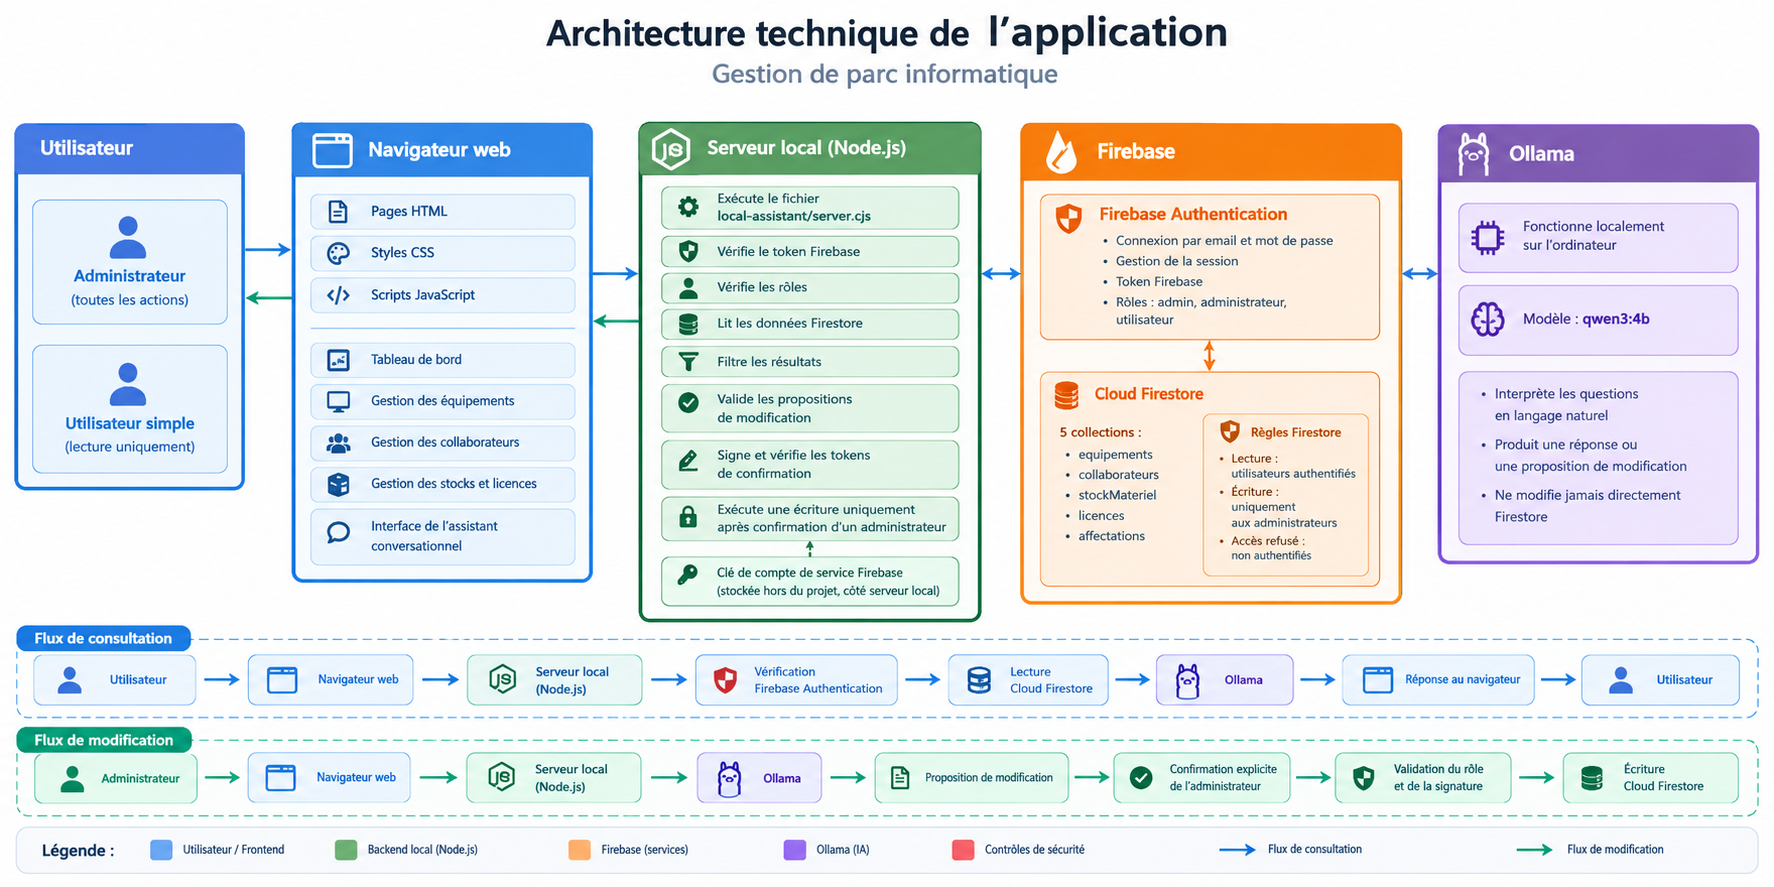
\includegraphics[width=\textwidth,height=0.72\textheight,keepaspectratio]{architecture-systeme.png}
    \caption{Architecture technique de l’application de gestion du parc informatique}
    \label{fig:architecture-application}
\end{figure}

\section*{Annexe D. Résultats détaillés des tests automatisés}
\phantomsection
\addcontentsline{toc}{section}{Annexe D. Résultats détaillés des tests automatisés}

\noindent Cette annexe détaille les six tests automatisés présentés au chapitre 5. Trois tests portent sur le cycle de vie des affectations dans \texttt{tests/assignment-lifecycle.test.mjs}, et trois autres sur les rôles et la validation des propositions dans \texttt{functions/assistant-core.test.cjs}.

\begin{longtable}{|p{0.9cm}|p{4.6cm}|p{6.1cm}|p{1.7cm}|}
    \caption{Cas de tests automatisés et résultats obtenus}
    \label{tab:annexe-tests-detail}\\
    \hline
    \textbf{ID} & \textbf{Cas testé} & \textbf{Résultat attendu} & \textbf{État} \\
    \hline
    \endfirsthead
    \hline
    \textbf{ID} & \textbf{Cas testé} & \textbf{Résultat attendu} & \textbf{État} \\
    \hline
    \endhead
    A-01 & Réaffectation d’un équipement déjà attribué & L’affectation précédente est clôturée et une nouvelle affectation active est créée avec les dates et identifiants attendus. & Réussi \\
    \hline
    A-02 & Compatibilité avec les noms de champs français utilisés dans Firestore & Les champs français sont interprétés correctement et le changement d’affectation produit les données attendues. & Réussi \\
    \hline
    A-03 & Détection de plusieurs affectations actives pour un équipement & L’état incohérent est refusé par la validation. & Réussi \\
    \hline
    S-01 & Reconnaissance des rôles et contrôle d’accès & Les rôles administrateurs sont reconnus ; un utilisateur simple n’est pas autorisé à agir comme administrateur. & Réussi \\
    \hline
    S-02 & Signature et vérification d’une proposition & Une proposition signée est vérifiée pour le bon utilisateur ; toute modification du token est refusée. & Réussi \\
    \hline
    S-03 & Contrôle des champs et collections autorisés & Les champs sensibles et les modifications non supportées, dont celles de la collection \texttt{affectations}, sont refusés. & Réussi \\
    \hline
\end{longtable}

\noindent L’exécution des tests est reproductible depuis la racine du projet avec les commandes suivantes :

\begin{minted}[fontsize=\small,breaklines,frame=single]{text}
node --test tests/assignment-lifecycle.test.mjs
node --test functions/assistant-core.test.cjs
\end{minted}

\noindent Ces tests couvrent la logique métier des affectations et le cœur de validation de l’assistant. Les scénarios fonctionnels réalisés dans le navigateur et les tests d’intégration avec Firebase ou Ollama sont décrits séparément au chapitre 5.

\end{document}